\documentclass[a4paper,10pt]{article}

% Lenguaje
\usepackage[spanish]{babel}
\usepackage[utf8]{inputenc}
\setlength{\parindent}{0pt}

% Ajustes documento
\usepackage{geometry}
\geometry{left=3cm,right=3cm,top=3cm,bottom=3cm,headheight=1cm,headsep=0.5cm}
\usepackage{enumitem}

\usepackage[table,xcdraw]{xcolor}
\usepackage{hyperref}
\hypersetup{
    colorlinks=true,
    linkcolor=[rgb]{0.149 0 0.3216},
    filecolor=magenta,      
    urlcolor=blue,
    citecolor=blue,
}
\urlstyle{same}

\usepackage{amsmath}

% Incluir apéndices
\usepackage[toc,page]{appendix}

% Incluir gráficos
\usepackage{graphicx}
\usepackage{subcaption}
\usepackage{float}

% Incluir código
\usepackage{listings}

\definecolor{codegreen}{rgb}{0,0.6,0}
\definecolor{codegray}{rgb}{0.5,0.5,0.5}
\definecolor{codepurple}{rgb}{0.58,0,0.82}
\definecolor{backcolour}{rgb}{0.95,0.95,0.92}

\lstdefinestyle{mystyle}{
  language=bash,
  backgroundcolor=\color{backcolour},   
  commentstyle=\color{codegreen},
  keywordstyle=\color{magenta},
  numberstyle=\tiny\color{codegray},
  stringstyle=\color{codepurple},
  basicstyle=\ttfamily\footnotesize,
  breakatwhitespace=false,         
  breaklines=true,                 
  captionpos=b,                    
  keepspaces=true,                 
  numbers=none,                   
  showspaces=false,                
  showstringspaces=false,
  showtabs=false,                  
  tabsize=2
}

\lstset{style=mystyle}

% Sangrado y espacio entre párrafos
\setlength{\parskip}{1em}
\setlength{\parindent}{1.5em}

% Portada
\title{Diseño y construcción de un sistema para adquisición y análisis
  del consumo energético en el hogar}
\author{Jesús Sánchez de Lechina Tejada}
\date{Junio 2020}

\begin{document}
\maketitle
\thispagestyle{empty}
\begin{center}
  \includegraphics[scale=0.4]{img/logo_ugr.pdf}
\end{center}

\newpage

\tableofcontents

\fontsize{12}{16}\selectfont

\newpage

\section{Introducción}\label{intro}

En este documento se recoge una descripción de mi Proyecto de Fin de
Grado, cuyo tema es: \textbf{Diseño y construcción de un sistema para
  adquisición y análisis del consumo energético en el hogar.}

Para ayudar en esta descripción se han reunido un conjunto de
explicaciones de los procesos empleados, análisis y el desarrollo de
algunas cuestiones relativas al proyecto.

\subsection{Objetivos y motivación}\label{objetivos}

El \textbf{principal objetivo} de este proyecto es doble. Del mismo modo que se
pretende diseñar un sistema para medir y controlar el consumo
energético en un hogar en sus distintos aspectos (hardware, software y
telecomunicaciones necesarias) se busca también hacer ver al lector
que, con ligeros conocimientos informáticos y la disposición por
aprender adecuada, cualquier individuo puede llegar a replicar el
sistema o incluso construir uno nuevo basándose en la descripción que
se ofrece de este diseño.

Analizando los requisitos del objetivo principal encontramos una
necesidad adicional: El sistema a diseñar requerirá una
infraestructura y un paradigma sobre el cual planificar el
proyecto. Esto resulta ser en realidad una ocasión para estudiar el
Internet de las Cosas, explicando qué es y cómo en la actualidad ya es
una solución a este problema aunque nos pueda parecer algo distante.

\subsection{Estructura del proyecto}\label{estructura}

\begin{itemize}
\item{\textbf{Sección~\ref{intro}:} Presentación del proyecto,
  motivación y objetivos del mismo. Se ofrece una introducción al
  Internet de las Cosas en el Apartado~\ref{internet-de-las-cosas},
  así se podrá conocer qué significa este término y qué aplicaciones
  tiene actualmente. Al final de esta sección se motiva el núcleo de
  este proyecto mediante una de las aplicaciones del Internet de las
  Cosas, la monitorización.}
  
\item{\textbf{Sección~\ref{revision-enchufes}:} En la
  Sección~\ref{revision-enchufes} se enlaza el concepto de Internet de
  las Cosas con la aplicación a los enchufes inteligentes, haciendo
  una pequeña taxonomía sobre estos y presentando algunos modelos
  actuales en el mercado con sus funcionalidades.}
  
\item{\textbf{Sección~\ref{arquitecturas-iot}:} Previo a la
  descripción en detalle de la construcción del sistema es conveniente
  conocer el contexto de las arquitecturas en el paradigma del
  Internet de las Cosas. Este es el objetivo que trata la
  Sección~\ref{arquitecturas-iot}, dar una visión sobre cómo se puede
  dar soporte al problema que nos planteamos.}
  
\item{\textbf{Sección~\ref{diseno-arquitectura}:} Una vez explicada
  esta arquitectura pasamos a, en la
  Sección~\ref{diseno-arquitectura}, profundizar en el uso que le
  hemos dado a distintos elementos de este paradigma para adecuarlos a
  las necesidades de nuestro proyecto. Explicando cómo hemos diseñado
  y construido todo el sistema desde la elección de sensores y
  microcontrolador hasta el diseño de la aplicación del usuario final
  pasando por toda la lógica de comunicación y almacenamiento de
  información intermedia.}

\item{\textbf{Sección~\ref{tests}:} Recopilación de pruebas que se han usado
  para verificar el correcto desarrollo del proyecto.}

\item{\textbf{Sección~\ref{conclusion}:} Reflexiones, conclusiones y
  análisis sobre el conjunto del resultado del proyecto.}
\end{itemize}

\newpage

\subsection{Internet de las Cosas}\label{internet-de-las-cosas}

Uno de los términos más recurrentes en el ámbito de la tecnología a día
de hoy es el de \textit{``Internet de las Cosas''} (en inglés, IoT, \textit{Internet of
Things}). Pero, puesto que el término puede resultar ambiguo, es
conveniente dar una definición sobre esta que permita esclarecer el
concepto.

El Internet de las Cosas es un paradigma tecnológico en sí mismo.
Desglosando el concepto vemos que reúne dos tecnologías. Por un lado
parte de ``las cosas'', que abarca desde los dispositivos y
electrodomésticos que podemos encontrar en nuestro día a día; que tienen
una funcionalidad en sí misma (p.ej.\ una televisión, un frigorífico),
hasta incluso podemos abstraer a personas o animales (una persona con un
marcapasos, un ave con un geolocalizador u otros
ejemplos\cite{iotagendawebsiteWhatInternetThings}). A estas ``cosas''
se les añade el término
``Internet'', que no es más que una abstracción de la conectividad que
permite dotar a las cosas de comunicación con el exterior, extendiendo
sus funcionalidades sin privarlas de su cometido original. Esta es
su principal característica, la posibilidad de comunicación con otras
``cosas'' mediante internet y sin la necesidad de intervención humana.

La idea que trasciende de esto es que cualquier cosa o dispositivo que
usemos habitualmente puede conectarse a una red, a internet. Haciendo
que, en términos de redes, un dispositivo IoT se pueda equiparar a un
ordenador convencional.

\subsubsection{¿Qué es un dispositivo
IoT?}\label{quuxe9-es-un-dispositivo-iot}

En el símil anterior hemos adelantado el concepto de dispositivo IoT sin
llegar a definirlo completamente. A continuación explicaremos qué es
concretamente un dispositivo IoT y qué lo diferencia de otras ``cosas''.

Un dispositivo IoT es una entidad (objeto, o incluso animales o
personas) que tiene una funcionalidad en sí misma y a la cual dotamos de
una capacidad de conexión y telecomunicación. De modo que sea capaz de,
por sí misma, comunicarse con otros dispositivos en su entorno dotados
de esta misma capacidad.

Los beneficios que podemos obtener de este paradigma se pueden aplicar
en muchas áreas\cite{vongsingthongs.;smanchats.IoTExamplesSuranaree},
por ejemplo:

\begin{itemize}
\item
  Logística: Rastreo de envíos por correo o estado del stock en
  almacenes automatizando lectura de los items mediante WiFi.
\item
  Transporte: Gestión automática de rutas por GPS;\ captura y procesado
  de infracciones de velocidad.
\item
  Salud: Desde una pulsera que capte tus hábitos de vida hasta
  la supervisión de personas ancianas que viven solas.
\item
  Monitorización: Desde instalación de sensores en un bosque para medir
  datos de contaminación hasta medir en un hogar el consumo de un
  electrodoméstico.
\end{itemize}

Este último ejemplo es justo la motivación de nuestro trabajo. Podemos
usar esta tecnología para crear un \textbf{enchufe inteligente} que
nos permita saber nuestro consumo eléctrico y controlar el uso que le
damos.

\newpage

\section{Revisión de enchufes inteligentes existentes en el
mercado}\label{revision-enchufes}

\subsection{¿Qué es un enchufe? Tipos de
enchufe}\label{tipos-de-enchufe}

Un enchufe es una fuente de alimentación entre sistemas eléctricos. En
este proyecto trataremos los enchufes dentro del ámbito doméstico o
comercial frente al ámbito industrial, que tiende a trabajar con
voltajes de un orden muy superior.

Un enchufe en el ámbito doméstico permite la conexión entre un
dispositivo electrónico y la corriente alterna para la alimentación de
este dispositivo.

Estos trabajan con unos voltajes entre 100V y
240V.\cite{iecIECWorldPlugs} El tipo de enchufe, voltaje y frecuencia
usados en una región geográfica vienen determinados por un convenio
fijado por el gobierno de esa zona.

Por razones históricas\cite{nuevatribunaOrigenFrecuenciasElectricas}
no existe una estandarización. Generalmente las zonas que se han
desarrollado con una mayor influencia entre los países que la
conforman tienden a compartir el mismo tipo de enchufe, por ejemplo el
más frecuentemente usado en la Unión Europea es distinto del usado en
Reino Unido a pesar de compartir las propiedades de frecuencia y
potencial eléctrico y situarse geográficamente más cercanos. Otras
regiones más distantes como Japón o Estados Unidos de América usan
enchufes con características distintas a ambas. Se ofrecen algunos
ejemplos de las propiedades de los enchufes por países en el
Cuadro~\ref{table:enchufes-paises}.

\begin{table}[H]
  \centering
  \begin{tabular}{lll}
    \rowcolor[HTML]{DAE8FC} 
    País      & Potencial  Eléctrico & Frecuencia \\
    Indonesia & 110V, 220V           & 50Hz       \\
    \rowcolor[HTML]{F8FF00} 
    España    & 230V                 & 50Hz       \\
    Reino Unido & 230V               & 50Hz       \\
    México    & 127V                 & 60Hz       \\
    E.E.U.U.  & 120V                 & 60Hz       \\
    Japón     & 100V                 & 50Hz, 60Hz \\
    Marruecos & 127V, 220V           & 50Hz      
  \end{tabular}
  \caption{Distintas zonas utilizan enchufes con distintas
    características, a pesar de en algunos casos tener el mismo
    potencial eléctrico y frecuencia}\label{table:enchufes-paises}
\end{table}

Trabajaremos con el tipo de enchufe usado en España, que cuenta con un
potencial de 230V y una frecuencia de 50Hz\cite{IECWorldPlugs}.

\newpage

\subsection{¿Qué es un enchufe
inteligente?}\label{que-es-un-enchufe-inteligente}

Un enchufe inteligente extiende esta definición de enchufe. Actuando
como una interfaz que permite añadir un amplio abanico de
funcionalidades relativas al manejo y supervisión de estos dispositivos
externos. Dotándole de las ventajas de la conectividad.

Esto encaja con la definición de dispositivo IoT que mencionábamos
previamente. Un objeto cotidiano que ha sido dotado de la capacidad de
comunicación con otros dispositivos.

\subsection{Funcionalidades comunes que ofertan los enchufes
electrónicos
actualmente}\label{funcionalidades-comunes-que-ofertan-los-enchufes-electruxf3nicos-actualmente}

\subsubsection{Monitorización:}\label{monitorizaciuxf3n}

Supervisar el uso de energía: Esto permite establecer un control sobre
su uso, realizar estimaciones sobre el coste o incluso notificar frente
a anomalías como el consumo en horarios no esperados o picos de voltaje.

\subsubsection{Control:}\label{control}

Manejar tus dispositivos de manera remota, programar el horario de
funcionamiento de estos o la manera en la que funcionan son solo algunas
de las opciones; destacando la posibilidad de integración con otros
dispositivos que proporcionen una mayor accesibilidad (p.ej.\ la interfaz
de voz de un asistente de móvil).

\newpage

\subsection{Tipos de enchufes}\label{tipos-de-enchufes}

Atendiendo a sus características más distintivas podemos hacer una
clasificación (no excluyente) de:

\begin{itemize}
\item
  Enchufes inteligentes (E.I.) por control remoto (WiFi, bluetooth,
  infrarrojos u otros tipos de señales electromagnéticas).
\item
  E.I. programables, aquellos que permiten la programación temporal de eventos.
\item
  E.I. de regletas, aquellos que permiten tratar con varios
  dispositivos simultáneamente en un mismo enchufe.
\end{itemize}

\subsection{Modelos en el mercado}\label{modelos-en-el-mercado}

La comercialización de este producto está muy extendida, proporcionando
una amplia oferta de productos los cuales podemos recoger bajo la
clasificación previa:

\begin{itemize}
\item
  \textbf{Programación temporal:} Permiten la ejecución de tareas a horas
  concretas del día. Por ejemplo:
  \href{https://web.archive.org/web/20191111121153/https://www.amazon.es/Garza-Power-Temporizador-anal\%C3\%B3gico-programaci\%C3\%B3n/dp/B00URUVDW2/}{Garza
  400603 (analógico)} (Figura~\ref{fig:enchufe-programable-analogico}),
  \href{https://web.archive.org/web/20191112121450/https://www.amazon.es/dp/B00ZJ1LQDK}{Orbegozo
    PG 20 (digital)} (Figura~\ref{fig:enchufe-programable-digital}).
\item
  \textbf{Control remoto:} Se pueden controlar con mando a distancia, a través de
  una app o con control por voz. Por ejemplo:
  \href{https://web.archive.org/web/20191112130933/https://www.amazon.es/dp/B06W586CDZ}{TP-Link
  HS100} (Figura~\ref{fig:enchufe-remoto}) o la
  \href{https://web.archive.org/web/20191116174434/https://www.amazon.es/dp/B07DJ2G1CW}{Regleta
  Xiaomi} (Figura~\ref{fig:enchufe-regleta}), que es un ejemplo
  de intersección entre E.I. de regleta y por control remoto.
\end{itemize}

\begin{figure}[H]
  \centering
  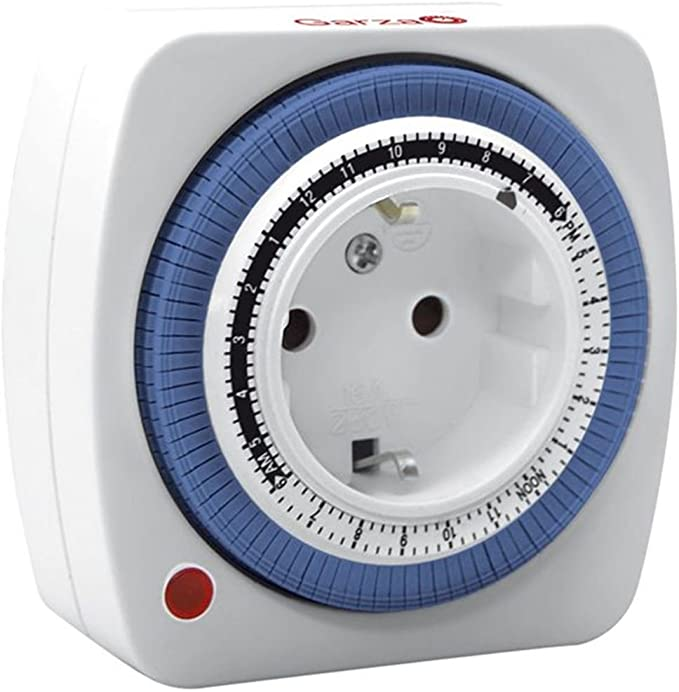
\includegraphics[width=0.5\textwidth]{img/enchufe_programable_analogico.jpg}
  \caption{Enchufe programable analógico Garza 400603. Imagen de~\cite{amazonwebsiteGarza400603Temporizador}}\label{fig:enchufe-programable-analogico}
\end{figure}

\begin{figure}
  \centering
  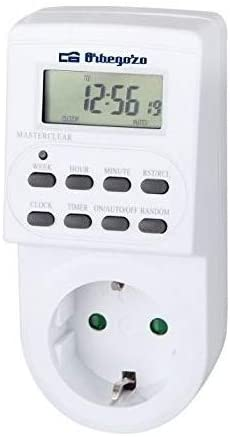
\includegraphics[width=0.3\textwidth]{img/enchufe_programable_digital.jpg}
  \caption{Enchufe programable digital Orbegozo PG20. Imagen de~\cite{amazonwebsiteOrbegozoPG202019}}\label{fig:enchufe-programable-digital}
\end{figure}

\begin{figure}
  \centering
  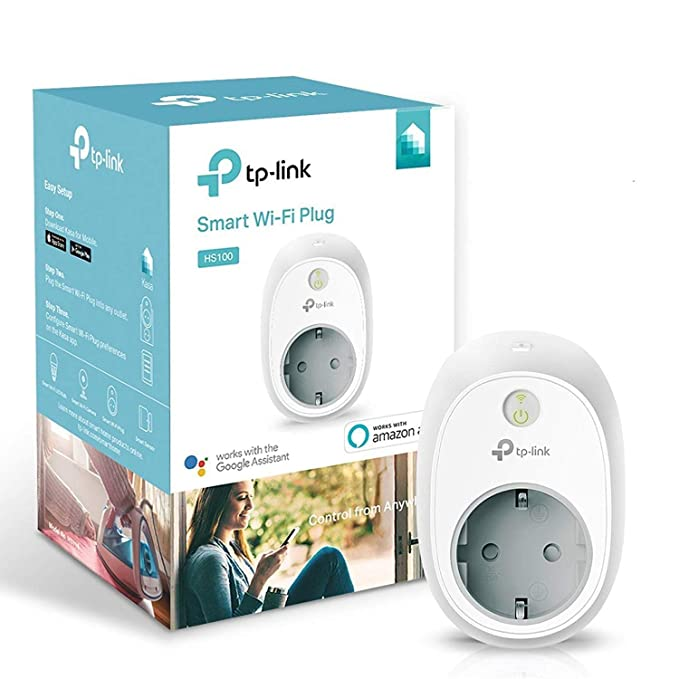
\includegraphics[width=0.5\textwidth]{img/enchufe_remoto.jpg}
  \caption{Enchufe por control remoto TP-Link HS100. Imagen de~\cite{amazonwebsiteTPLinkHS100Enchufe}}\label{fig:enchufe-remoto}
\end{figure}

\begin{figure}[H]
  \centering
  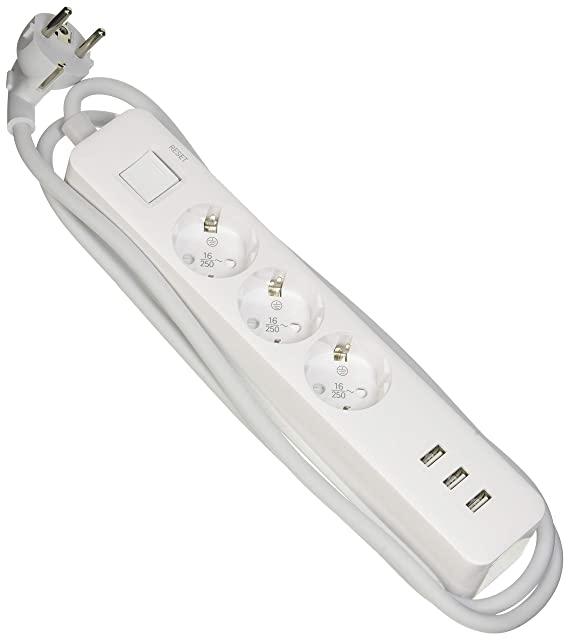
\includegraphics[width=0.5\textwidth]{img/enchufe_regleta.jpg}
  \caption{Enchufe regleta por control remoto Xiaomi. Imagen
    de~\cite{amazonwebsiteXiaomi18082Regleta2019}}\label{fig:enchufe-regleta}
\end{figure}

\newpage

\section{Arquitecturas IoT}\label{arquitecturas-iot}

El paradigma de IoT viene a integrarse entre los mecanismos
convencionales y el resto de redes. En sus primeros pasos se adaptaron
sus diseños a las necesidades de estos sistemas. Pero según fue
desarrollándose fueron naciendo algunas arquitecturas que ayudaban a
definir y a trabajar mejor con los requisitos de estos nuevos sistemas.

Existen diferentes arquitecturas en la actualidad, que difieren en el
enfoque que le dan a ciertos campos. Dos de los más conocidos son IoT-A
e IIRA.\ Siendo el primero el más extendido desde su lanzamiento en
2012.\cite{weyrichReferenceArchitecturesInternet2016}

Algunos campos de comparación entre arquitecturas de IoT son\cite{atzoriInternetThingsSurvey2010}:

\begin{itemize}
\item
  El enfoque particular a casos de negocio frente a conceptos generales.
\item
  Orientación a Internet: Si se introducen nuevos protocolos y se
  adaptan los ya existentes a sus necesidades.
\item
  Tipo de dispositivo sobre el cual se orienta (como sensores o
  actuadores).
\end{itemize}

Estas arquitecturas coinciden en la definición de capas de manera
análoga a TCP/IP u
OSI\cite{weyrichReferenceArchitecturesInternet2016}, pero adaptándolas
a las necesidades del IoT. Ante las diversas clasificaciones en
múltiples capas se puede encontrar una similitud entre ellas que
permite generalizar en 3 capas principales: Percepción, asociada a los
dispositivos físicos, consistente en sensores; capa de red, encargada
de transmitir información entre sensores y sistemas procesadores
finales; y capa de aplicación, para el proceso final de la
información\cite{khanFutureInternetInternet2012}.

Para conocer cómo se produce la comunicación a distintos niveles de la
arquitectura es necesario analizar sus protocolos.

\subsection{Protocolos}\label{subsec:protocolos}

Dos ordenadores convencionales necesitan una pila de protocolos para que
puedan transmitir información a las distintas capas que conforman la
comunicación. Ante los requisitos que surgían con los dispositivos IoT,
emergían también protocolos que daban respuesta a estos. Estableciéndose
así una pila de protocolos de red especializada para IoT.

A fin de permitir estas comunicaciones de manera liviana es necesario
alguna tecnología a \textbf{nivel físico} que pueda solventar el
problema de la saturación del espectro de frecuencias, algunas
propuestas se basan en aprovechar el ruido blanco (frecuencias no
usadas en el espectro de radio)\cite{tempertonTVWhiteSpace2015}.  En
la \textbf{capa de enlace} se encuentra
6LoWPAN\cite{schumacherIPv6LowPowerWireless} para conectar los
dispositivos a una red IP, dicha red ha de ser del tipo IPv6
(\textbf{capa de red}) para dar soporte a la escalabilidad.

En la \textbf{capa de aplicación} existen alternativas para
proporcionar un transporte de datos con baja sobrecarga en la
comunicación. Algunas de estas opciones\cite{al-fuqahaInternetThingsSurvey2015}
son: \textbf{CoAP}
(Constrained Application Protocol), usado como un protocolo web basado
en \textit{REST}\cite{WebServicesArchitecture}; \textbf{XMPP}
(Extensible Messaging and Presence Protocol), usado especialmente en
mensajería; \textbf{DDS} (Data Distribution Service), especializado en
aplicaciones de tiempo real y con alta disponibilidad; o \textbf{MQTT}
(Message Queue Telemetry Transport), para conectar dispositivos
embebidos con aplicaciones y middleware.

Esta es una de las decisiones que más afecta al diseño, pues el resto
del diseño de la arquitectura se ve afectado por ello.

\subsection{Modelos de interconexión de
red}\label{modelos-de-interconexiuxf3n-de-red}

De acuerdo a la topología de la red, el modo en el que se conectan los
dispositivos involucrados, reconocen ocho tipos básicos de modelos de
interconexión.\cite{bicsiNetworkDesignBasics2002}

\begin{itemize}
\item{Punto a punto: Dos dispositivos finales se perciben directamente
  conectados entre sí.}
\item{Cadena Margarita: Se conecta en serie cada computador al
  siguiente, los mensajes se retransmiten durante toda la cadena.}
\item{Bus: Todos los dispositivos están conectados entre sí usando
  un cable central. Esto implica una difusión de cada mensaje a
  todos los nodos. Es más usual en redes locales.}
\item{Estrella: Un conjunto de nodos periféricos se conectan con un
  nodo central que actúa como servidor.}
\item{Anillo: Similar a una topología de “cadena margarita” donde
  existe un único bucle y la comunicación se realiza en un único
  sentido.}
\item{Malla: Los dispositivos se conectan de muchos a muchos, puede
  ser completamente conectada o parcialmente conectada si todos los
  nodos pueden o no encontrarse conectados entre sí. Esta categoría se
  puede identificar con un grafo, y como tal incluye a la topología de
  árbol, un tipo particular de grafo.}
\item{Híbrida: Aquellas que combinan varias topologías básicas para
  formar otras más complejas.}
\end{itemize}


\begin{figure}[H]
  \centering
  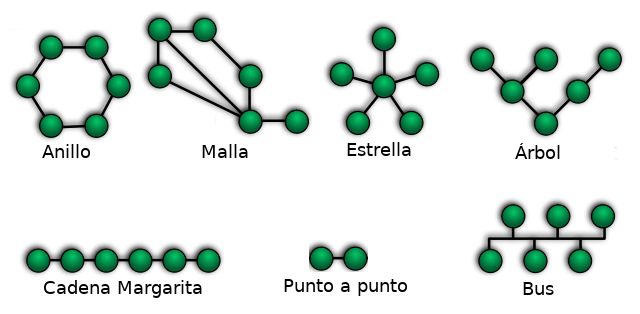
\includegraphics[width=0.8\textwidth]{img/NetworkTopologies_esp.png}
  \caption{Visualización de algunas topologías básicas de red}\label{fig:topologias-red}
\end{figure}



El modelo de interconexión de red de un sistema no es inherente al
Internet de las Cosas, es una cuestión recurrente en cualquier diseño
de una red de telecomunicación y cuya decisión se realiza en tanto a
las necesidades del sistema. Por ejemplo un modelo de malla consta de
una mayor complejidad en las comunicaciones que una de anillo, pero
este puede dificultar las comunicaciones entre distintos nodos. Una
arquitectura de estrella simplifica este problema pero se vuelve
dependiente de que el nodo central se encuentre siempre operativo.

\newpage

\section{Diseño de la arquitectura de nuestro
sistema}\label{diseno-arquitectura}

\subsection{Descripción general}\label{descripcion-general}

Nuestro enchufe inteligente recoge mediante el sensor SCT013 la
corriente que requiere el dispositivo conectado. En el módulo ESP32 se
realiza el cálculo del consumo en Vatios y se emite hacia nuestro
servidor, una Raspberry Pi con Mosquitto haciendo uso del protocolo de
comunicación MQTT, de donde se podrá consultar desde una aplicación
externa para supervisar el consumo y manipular el enchufe.

\begin{figure}[H]
  \centering
  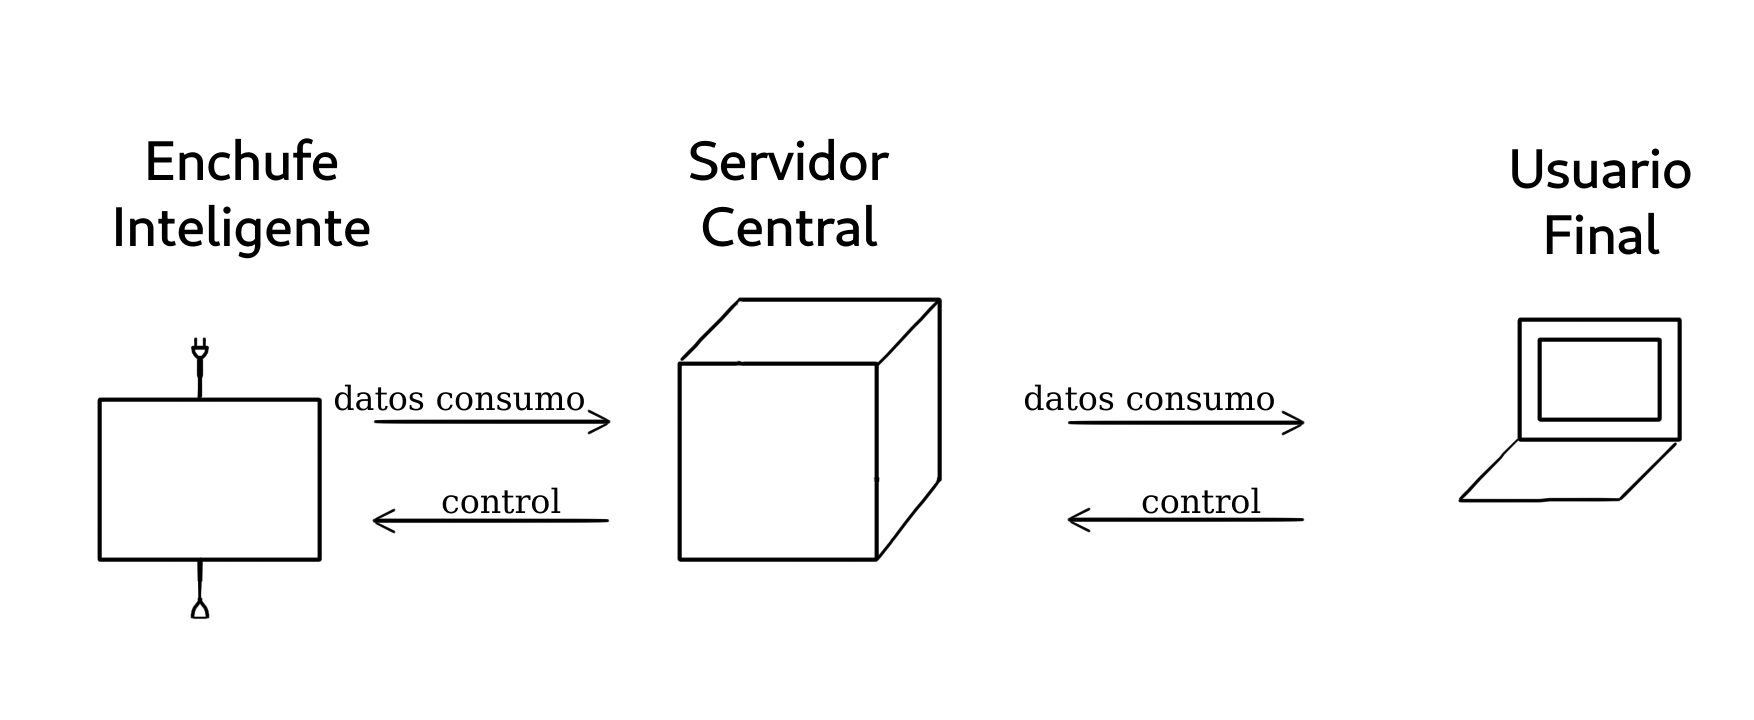
\includegraphics[width=0.8\textwidth]{img/esquema_basico_sistema.png}
  \caption{Representación simplificada del sistema y sus comunicaciones
    principales.}\label{fig:esquema_basico}
\end{figure}


Como mencionábamos en la Sección~\ref{arquitecturas-iot},
habitualmente las arquitecturas IoT se engloban bajo tres capas. La de
percepción, nuestro sensor que recoge los datos; la capa de red, el
uso de MQTT para gestionar las comunicaciones de manera liviana (sobre
TCP/IP) y la capa de aplicación, que permite el procesamiento,
manipulación y visualización por parte del usuario del sistema.

\newpage

\subsection{Modelo de red usado}\label{modelo-de-red-usado}

La topología de red usada en este proyecto es el modelo en
estrella. En el centro se encuentra nuestro servidor que se encarga de
gestionar tanto la información de los sensores como de otorgar la
visualización y manejo sobre los enchufes a los usuarios. En los
extremos se encontrarían tanto los enchufes inteligentes como los
usuarios desde sus aplicaciones.

\begin{figure}[H]
  \centering
  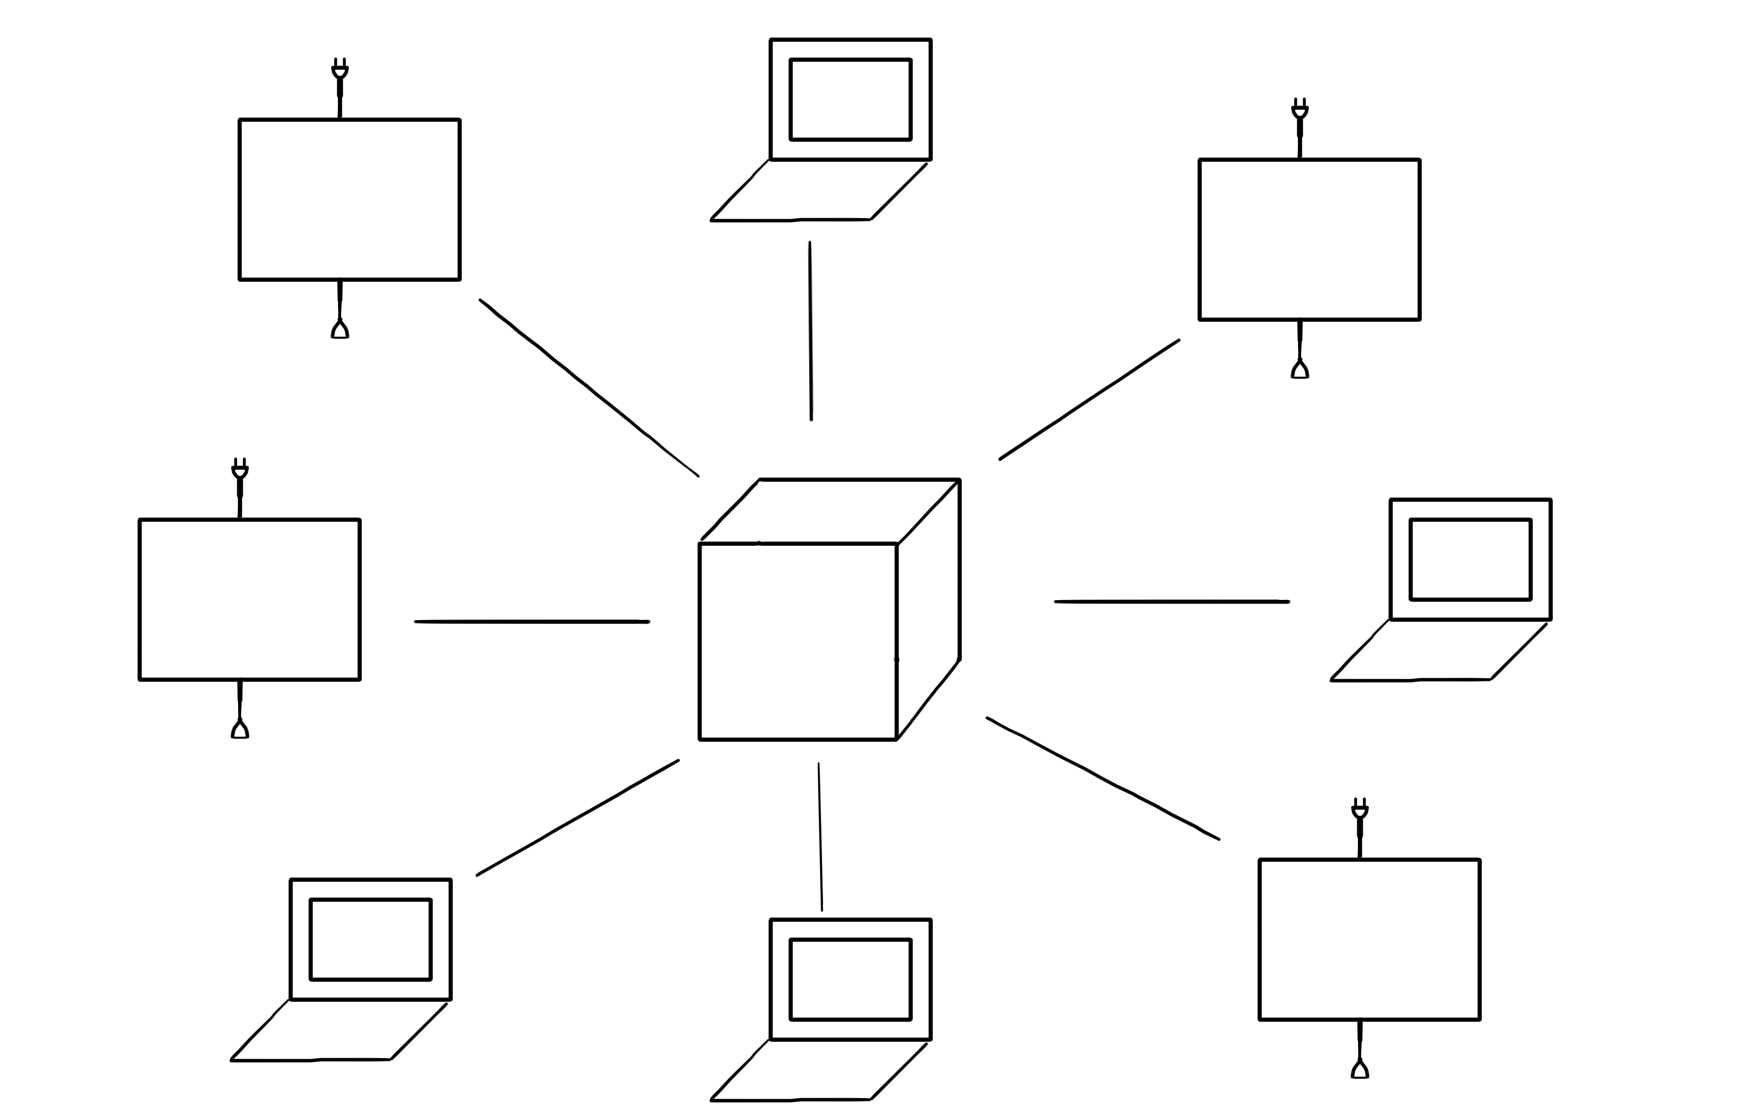
\includegraphics[width=0.8\textwidth]{img/esquema_estrella.png}
  \caption{Topología del sistema}\label{fig:esquema_estrella}
\end{figure}


Se ha decidido utilizar este modelo tanto por su versatilidad como
simplicidad para conectar los nodos periféricos al servidor central.

\newpage

\subsection{Protocolo MQTT}\label{protocolo-mqtt}

De los protocolos previamente mencionados [\ref{subsec:protocolos}]
optamos por utilizar MQTT por su facilidad de integración con
Mosquitto, un broker (agente intermediario) que implementa este
protocolo y cuya ligera carga le permite ejecutarse en servidores de
bajas prestaciones (Raspberry Pi, en nuestro caso).

MQTT utiliza el patrón de publicación/suscripción (publish-suscribe),
un publicador escribe sobre un tema (topic) del cual un suscriptor
lee. Está construido sobre TCP.

El tipo de comunicación en este protocolo es indicado en cada mensaje
en la cabecera del paquete. Proporciona mensajes para conexión
(CONNECT), desconexión (DISCONNECT), publicar en un tema (PUBLISH),
suscribirse/desuscribirse a un tema (SUBSCRIBE/UNSUSCRIBE) y otros
mensajes de control correspondientes a una respuesta ACK a los
anteriormente mencionados (pues está basado en
TCP).\cite{banksMQTTVersionEdited}

Todos los mensajes en MQTT se rigen bajo estas primitivas de
control. Todos los paquetes que usan para comunicarse se denomina
Paquete de control MQTT y tienen su propio formato como podemos
apreciar en el Cuadro~\ref{table:cabecera-mqtt}.

\begin{table}[H]
  \centering
  \begin{tabular}{|l|}
    \hline
    Cabecera fija: Presente en todos los paquetes de control   \\ \hline
    Cabecera variable: Presente en algunos paquetes de control \\ \hline
    Carga: Presente en algunos paquetes de control             \\ \hline
  \end{tabular}
  \caption{Estructura general de un paquete de control MQTT}\label{table:cabecera-mqtt}
\end{table}

En la cabecera fija se indica el tipo de mensaje de control y se
reservan algunos bits como indicadores, \textit{flags}, para indicar
parámetros como el QoS (\textit{Quality of Service}, garantías en el
modo de entrega del mensaje).

En la cabecera variable se indican otros contenidos, por ejemplo un
identificador de paquete cuando se establece un QoS que garantice la
entrega del mensaje.

En la sección correspondiente a la carga se transporta información que
complementa al mensaje de control. En un mensaje SUBSCRIBE se incluye
identificador, tema a suscribirse, usuario y contraseña si se
requiere, mientras que en un paquete PUBLISH en nuestro sistema
la carga sirve para que los enchufes inteligentes transmitan el
consumo que han calculado.

\newpage

\subsection{Diseño broker, publishers,
suscribers}\label{diseuxf1o-broker-publishers-suscribers}

Aunque existen otros subtipos de patrones publicador/suscriptor
basados en tipo o en contenido\cite{p.th.eugsterManyFacesPublish},
MQTT utiliza un modelo basado en temas.

Las principales componentes de este patrón son suscriptor, publicador
y el broker. Un dispositivo interesado se registra como suscriptor de
un tema y el broker se encargará de informarle cuando se publique algo
en el tema. El publicador actúa como un generador de información de
algún tema de interés. El broker es el intermediario que transmite a
los interesados, teniendo en cuenta además comprobaciones de seguridad
mediante autorización de publicadores y
suscriptores.\cite{al-fuqahaInternetThingsSurvey2015,hunkelerMQTTSPublishSubscribe2008}

Por este motivo, en este patrón pueden existir múltiples publicadores
y suscriptores mientras que es la entidad que actúa como broker la que
gestiona el flujo de comunicación. Un ejemplo general sobre esta
arquitectura basada en temas lo podemos encontrar en la
Figura~\ref{fig:arquitectura_pub_sub}. En ella unos sensores dotados
de conectividad, como nuestros enchufes inteligentes, se encargan de
publicar en unos temas una información determinada. Unos clientes
interesados se suscriben a los temas que sean de su interés para su
posterior uso.

\begin{figure}[H]
  \centering
  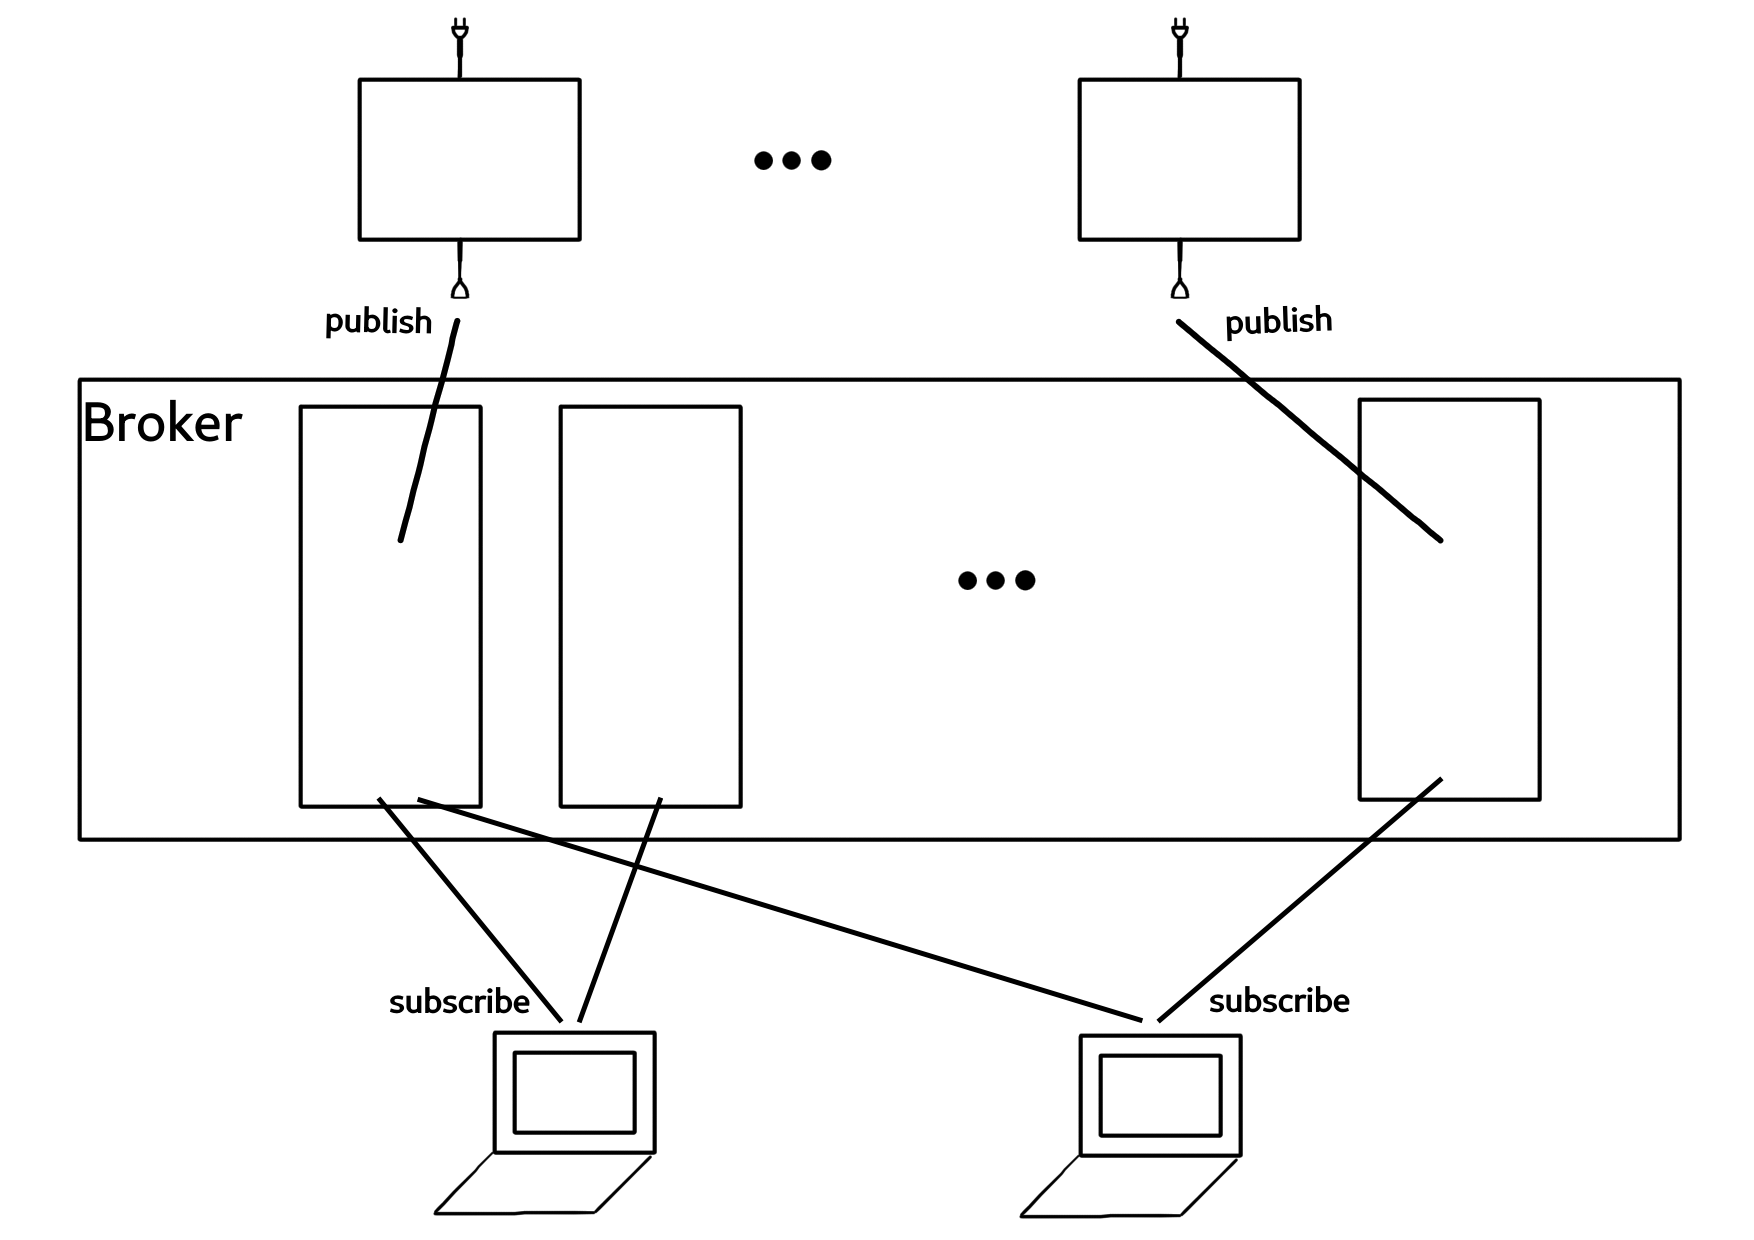
\includegraphics[width=0.8\textwidth]{img/arquitectura_pub_sub_ejemplo.png}
  \caption{Ejemplo genérico del uso de un broker.}\label{fig:arquitectura_pub_sub}
\end{figure}

La arquitectura que hemos diseñado en nuestro sistema sigue el mismo
patrón, pero se adapta al uso de diversos temas, tanto de consumo como
de control. En la Figura~\ref{fig:arquitectura_broker_sistema} podemos
ver cómo los enchufes inteligentes se encargan tanto de enviar como de
recibir información del broker. Publican la información relativa al
consumo de los dispositivos conectados en los temas de consumo y se
suscriben a los temas de control para que los usuarios finales puedan
manipular el estado de los enchufes.

\begin{figure}[H]
  \centering
  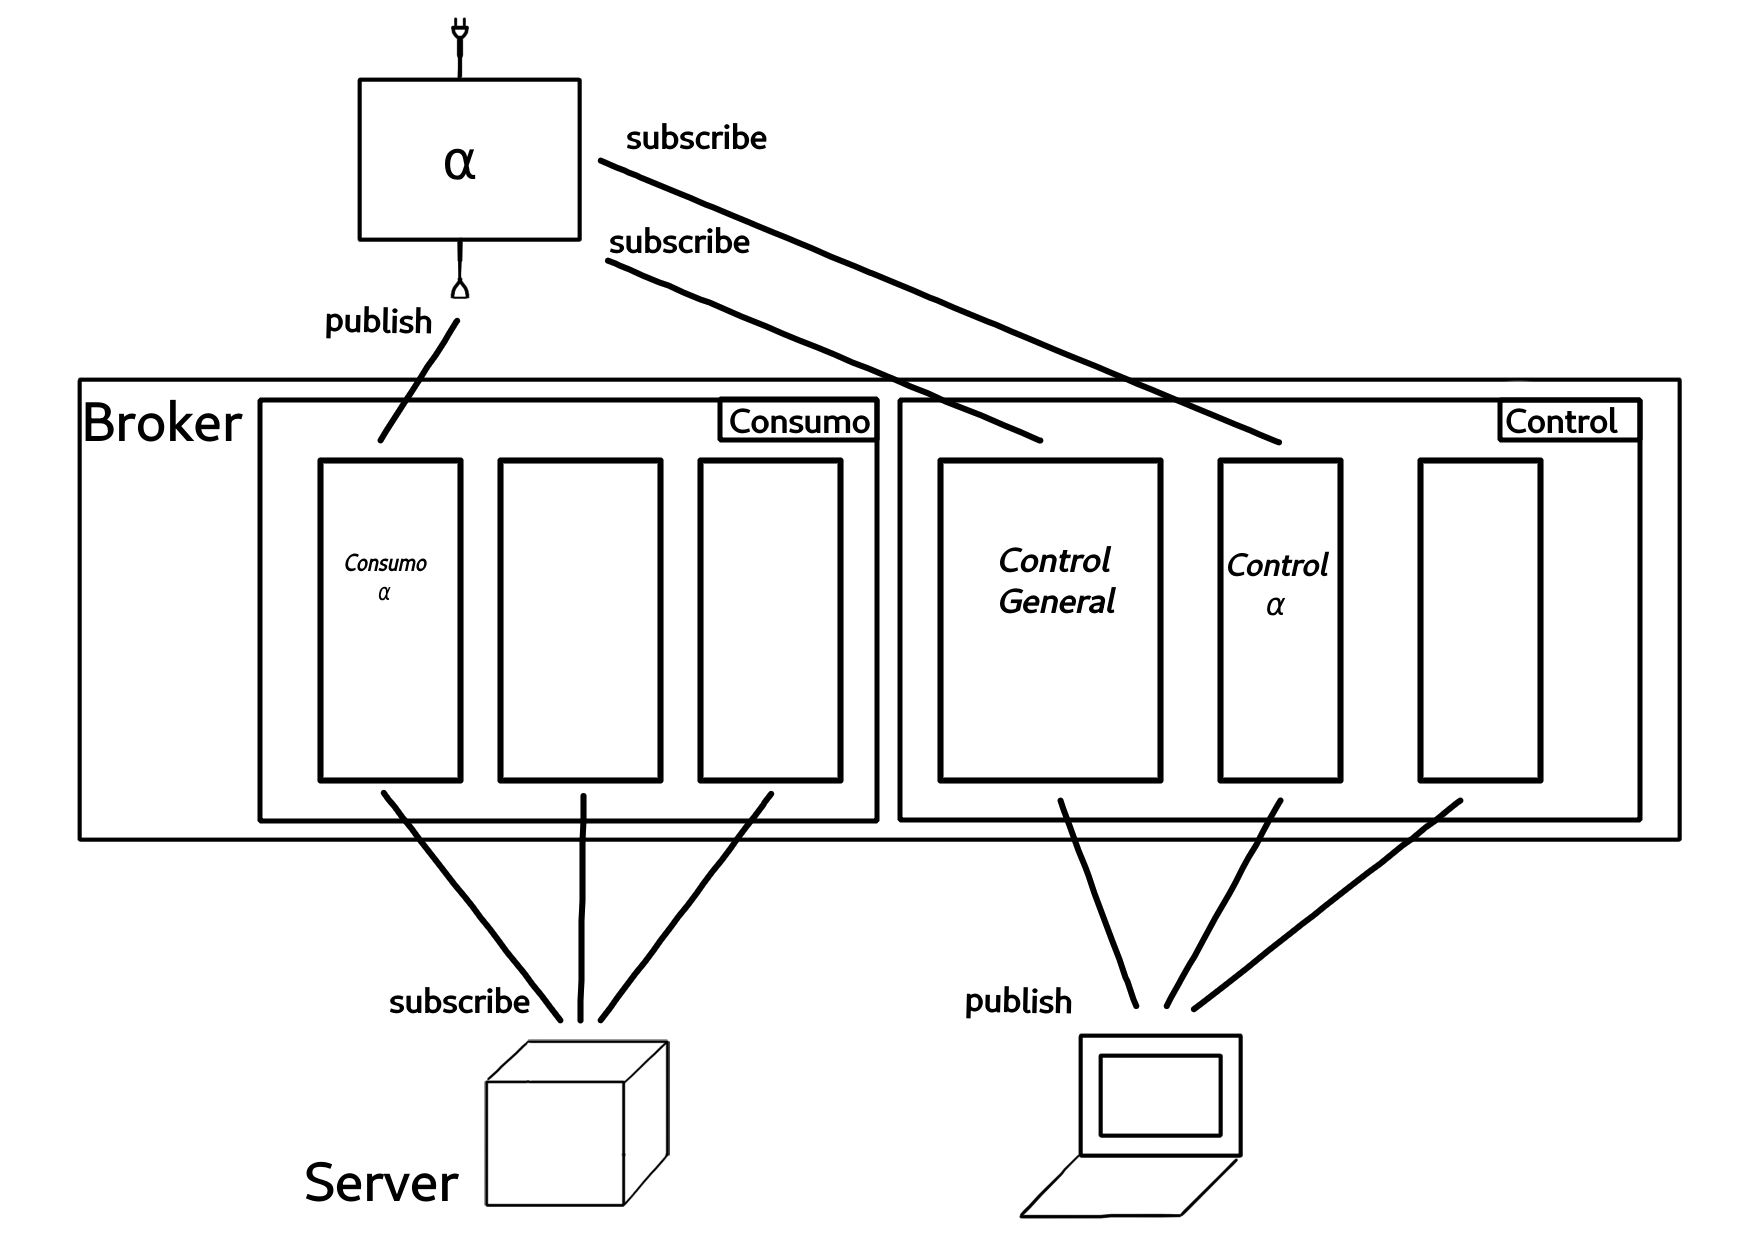
\includegraphics[width=0.8\textwidth]{img/arquitectura_broker_sistema.png}
  \caption{Comunicaciones MQTT en nuestro sistema.}\label{fig:arquitectura_broker_sistema}
\end{figure}

Es destacable de la Figura~\ref{fig:arquitectura_broker_sistema} que
sólo existe un suscriptor MQTT a los canales de consumo, el propio
servidor central. Esto sucede para que exista una única base de datos
centralizada y evitar problemas de inconsistencia en caso de que algún
cliente se caiga y se encuentren bases de datos con estados
distintos. La consulta de información relativa al consumo por parte
del usuario final se produce vía HTTP y se explicará con mayor
detenimiento en la Sección~\ref{subsubsec:consulta-api}.

MQTT define tres niveles de QoS para adaptarse a los requisitos del
sistema: 0 para una única entrega sin confirmación, 1 para al menos
una entrega donde se requiere una confirmación, 2 para exactamente una
entrega de mensaje utilizando una confirmación en 4 pasos
(\textit{four step handshake}). En definitiva a mayor QoS mayor
fiabilidad en el envío de mensajes a expensas de una mayor latencia y
requisitos de ancho de banda.

En nuestro sistema hemos optado por utilizar el QoS 0, pues la
información a transmitir es tolerante a pérdidas. Se envían mensajes
con el consumo con gran frecuencia y, por ser una serie temporal donde
todos los datos guardan una relación con los inmediatamente contiguos,
se puede realizar una estimación de valores perdidos por una
interpolación sin que esto repercuta negativamente en el análisis.

Todos los mensajes se pueden configurar para ser retenidos incluso
después de haber sido transmitidos a todos los suscriptores. Esto
resulta especialmente útil si aparece algún suscriptor en algún tema
que se actualice poco frecuentemente para que pueda acceder a la
información con la que trabajar lo antes posible.


\newpage

\subsubsection{Mosquitto}\label{subsubsec:broker_mosquitto}

El broker que usamos en nuestro diseño es
\textbf{Mosquitto}\cite{EclipseMosquitto}. Agente que implementa MQTT
v3.1.1, la versión de MQTT usada en este proyecto.

Uno de los requisitos más habituales en sistemas IoT es la integración
de manera ubicua de las componentes en el entorno del usuario. A
menudo esto implica utilizar sistemas compactos o embebidos con pocos
recursos. En nuestro caso utilizamos un servidor con recursos
limitados, una Raspberry Pi, por lo que resulta beneficioso utilizar
un broker tan ligero que no suponga una sobrecarga en el sistema.

Los temas en Mosquitto se disponen siguiendo una estructura jerárquica
similar a un sistema de archivos (\texttt{/RUTA/AL/TEMA}). En forma de
árbol. Permitiendo a un suscriptor suscribirse tanto a un tema
particular (nodo hoja) como a un nodo más general (cualquier nodo
interno).

En su estructura también guardan metainformación relativa al propio
broker: bytes enviados y recibidos, clientes conectados o mensajes
pendientes entre otros.

Otra utilidad de mosquitto es la capacidad de establecer
\textit{puentes}. Múltiples brokers pueden estar conectados con esta
funcionalidad. Esto es útil cuando se desea compartir información
entre distintas localizaciones pero no toda la información ha de ser
compartida.

Mosquitto permite numerosas opciones de configuración. Desde
autenticación, cifrado y retención de mensajes hasta cuestiones de registros
(\textit{logging}), conectividad o uso los recursos del sistema.


\newpage

\subsection{Enchufe}\label{subsec:enchufe}

De los tres subsistemas que componen el diseño de nuestro sistema
podríamos atribuirle el concepto de Enchufe Inteligente a este. Pues
es el encargado de realizar las lecturas del consumo energético del
dispositivo conectado, transmitir estas lecturas al servidor central y
manejar mediante el uso de un relé la alimentación del dispositivo
conectado para regular su uso.

El enchufe está compuesto por cuatro elementos principales:

\begin{itemize}
\item{\textbf{Módulo WiFi:} Microcontrolador
  ESP32\cite{ESP32SeriesDatasheet}. Núcleo del enchufe, encargado de
  ejecutar el programa principal que gestiona el manejo de lecturas y
  del relé. Dispone de funcionalidad WiFi para conectarse vía MQTT al
  servidor.}

\item{\textbf{Relé:} Tongling jqc-3ff-s-z, un relé de 5V que controla
  el paso de corriente por el dispositivo conectado cual interruptor y
  que es gestionado por el módulo ESP32.}

\item{\textbf{Sensor de corriente:} Sensor YHDC SCT013\-000
  CT\cite{SCT013000DatasheetPDF}. Un sensor de corriente no invasivo
  (basta con colocarlo alrededor del cable a medir) que actúa como un
  transformador de corriente. Transforma la corriente de entrada entre
  0 y 100 Amperios en otra de salida entre 0 y 50 miliAmperios que,
  mediante el uso de una resistencia de carga que convierta a un
  voltaje adecuado, el módulo es capaz de procesar.

  Los cables convencionales suelen estar compuestos por dos cables
  internos que conducen la corriente en sentido opuesto. Para evitar
  que se anulen las medidas el sensor se coloca en torno a uno de
  ellos. Además, es posible medir el sentido de la corriente para
  determinar si se está consumiendo o generando electricidad.}

\item{\textbf{Fuente de alimentación:} Una fuente de alimentación de
  5 Voltios y 2 Amperios para alimentar el módulo WiFi. Un conversor
  que toma la corriente alterna que llega al enchufe y alimenta al
  resto del circuito.}
\end{itemize}

\begin{figure}[H]
  \centering
  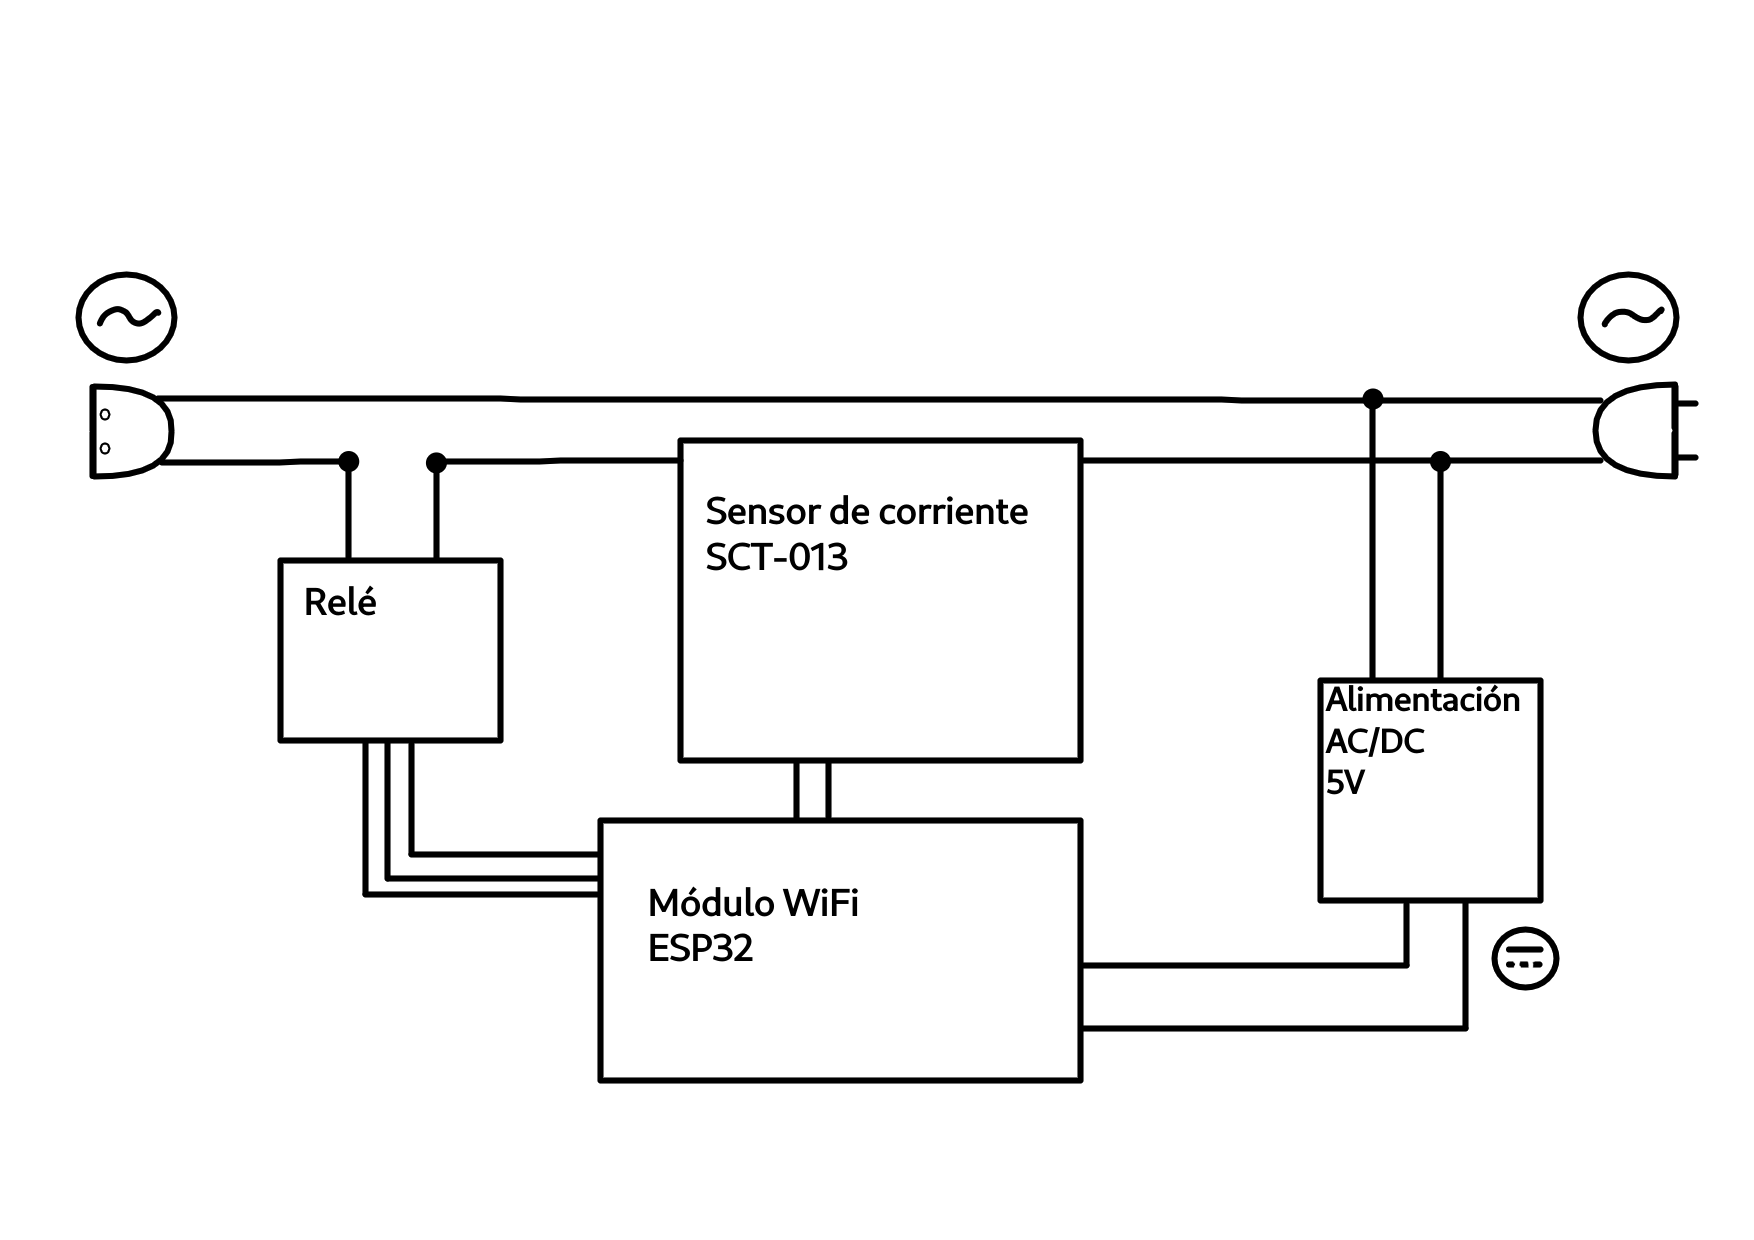
\includegraphics[width=0.9\textwidth]{img/esquema_enchufe_inteligente.png}
  \caption{Esquema del Enchufe Inteligente.}\label{fig:esquema-enchufe-inteligente}
\end{figure}

\subsubsection{Diseño y construcción del enchufe}

En un proceso de prueba y selección de componentes descartamos otras
opciones en el diseño de nuestro enchufe:

El microcontrolador Arduino UNO carecía de funcionalidad WiFi y el uso de módulos
externos requería alimentación extra. El ESP32 usado sí que disponía
de WiFi y era compatible con el resto de componentes, reduciendo así
la complejidad de este subsistema mientras otorgaba la misma funcionalidad.

\begin{figure}[H]
  \centering
  \begin{subfigure}{0.5\textwidth}
    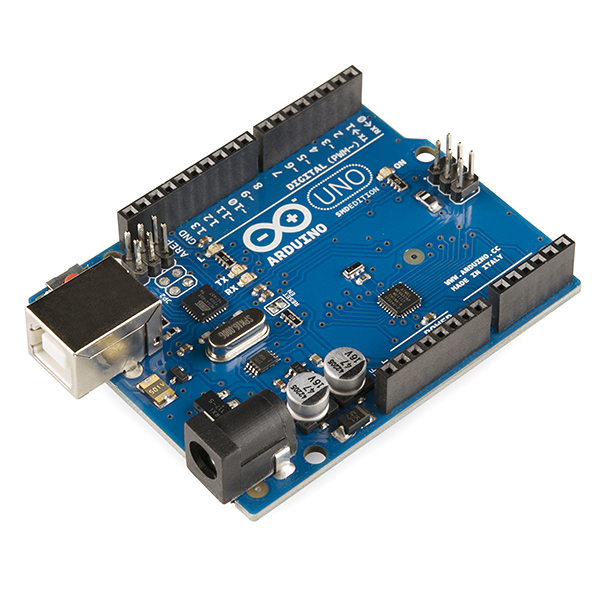
\includegraphics[width=0.9\linewidth, height=5cm]{img/arduino_uno.jpg} 
  \end{subfigure}
  \begin{subfigure}{0.49\textwidth}
    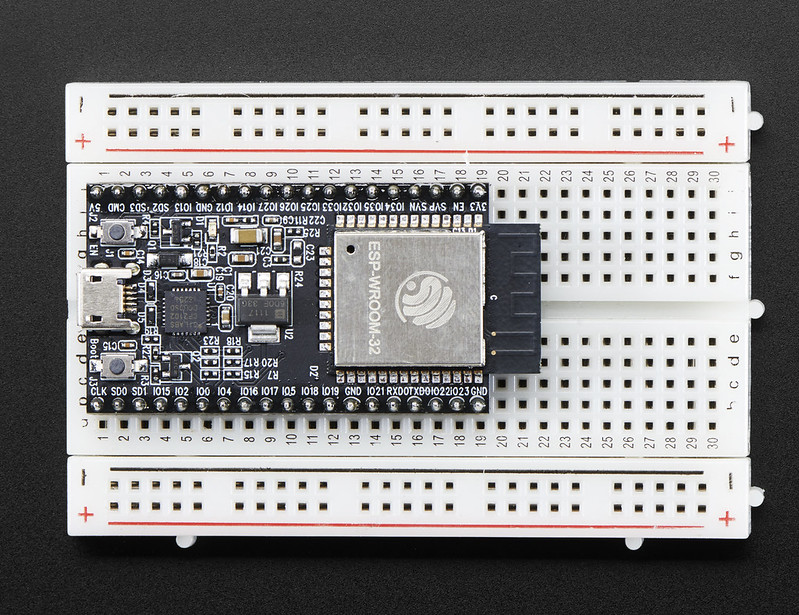
\includegraphics[width=1\linewidth, height=5cm]{img/esp32_image.jpg}
  \end{subfigure}  
  \caption{Arduino UNO, a la izquierda, imagen de~\cite{ArduinoR3}. A su derecha
    módulo ESP32, imagen de~\cite{industriesEspressifESP32Development2016}.}
\end{figure}

El sensor de corriente no invasivo fue seleccionado tras descartar el
sensor ACS712\cite{ACS712DatasheetPDF}. A pesar de realizar varias
pruebas con varios sensores para descartar que fuera defectuoso
descartamos el uso de esta componente. Este introducía ruido en las
lecturas, mostrando diferencias entre el consumo esperado y el
registrado para componentes eléctricas que conociéramos de antemano
(por ejemplo una bombilla).

En su lugar el sensor SCT013 fue más consistente en las lecturas y su
diseño no invasivo simplifica notoriamente las labores de
mantenimiento en caso de avería y reduce el riesgo en la instalación
al exponer menos componentes.

\begin{figure}[H]
  \centering
  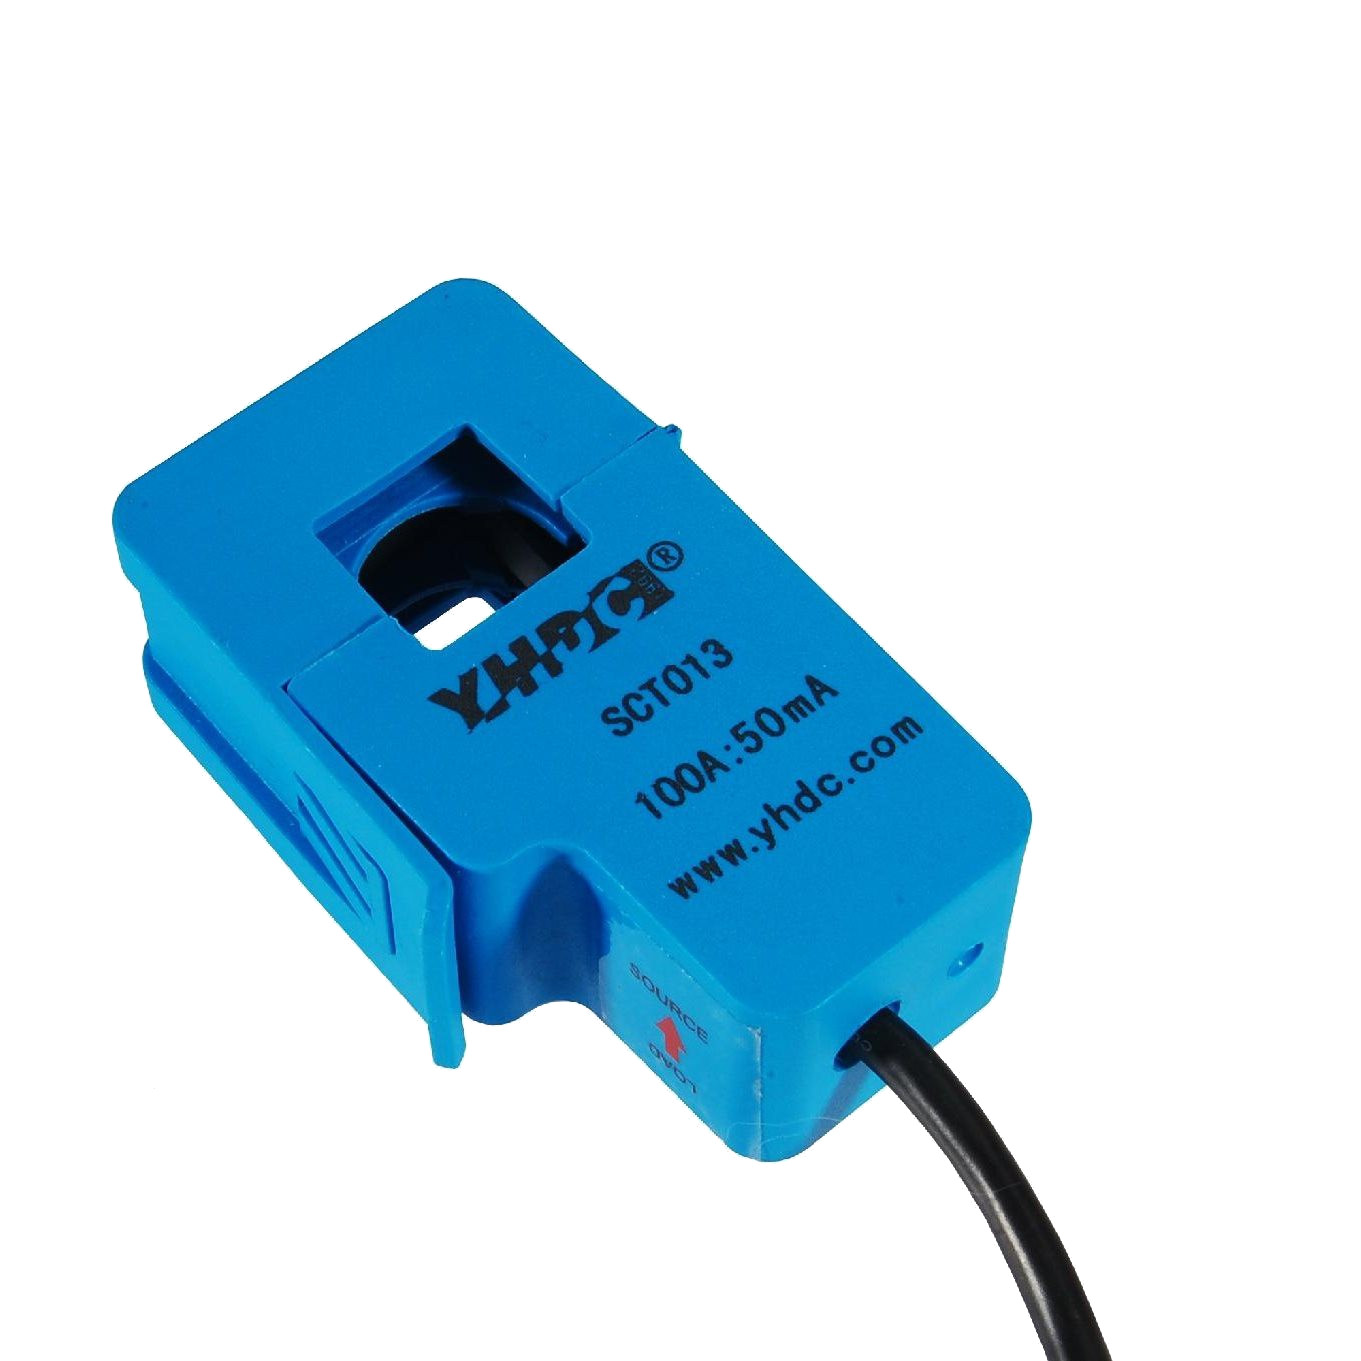
\includegraphics[width=0.8\textwidth]{img/sct013.png}
  \caption{Sensor de corriente no invasivo.}\label{fig:sct013}
\end{figure}



Tras esta selección procedimos a probar y, posteriormente, soldar el
enchufe a una placa base. A fin de minimizar el número de cruces entre
cables elaboramos el diseño visible en
la Figura~\ref{fig:placa-sup-arriba-abajo}. Este representa la vista superior de
la placa y cómo se disponen los cables y las componentes tanto por
encima como por debajo de la misma. Es conveniente indicar que cada
rectángulo representa un conjunto de pines que irán conectados a
alguna componente del sistema: El rectángulo GND, 5V a la fuente de
alimentación, el par In, Out la entrada y salida del sensor de
corriente y la tres-upla Vcc, Gnd y S a la alimentación y control del
relé.

\begin{figure}
  \centering
  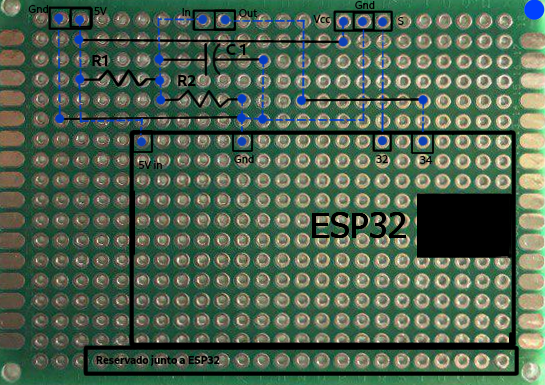
\includegraphics[width=0.8\textwidth]{img/dibujo_placa_vista_superior_arriba_y_abajo.png}
  \caption{Vista superior de la placa, en negro componentes y cableado
  de la parte anterior. En azul, de la parte posterior.}\label{fig:placa-sup-arriba-abajo}
\end{figure}

Hacemos uso del condensador $C1 = 10\mu F$ para absorber los
posibles picos de tensión, reducir el ruido en las lecturas y
garantizar calidad en las mismas.

Las resistencias $R1=R2=2k\Omega$ cumplen la función de un divisor de
tensión y de resistencia de carga para garantizar el voltaje operativo
del sensor de corriente y otorgar el rango de voltaje de salida esperado.

Para complementar esta visualización añadimos la parte posterior (trasera) de la
vista trasera de la placa (volteo vertical), Figura~\ref{fig:placa-tras-inf},
y la parte posterior de la vista superior, Figura~\ref{fig:placa-sup-inf}.

\begin{figure}
  \centering
  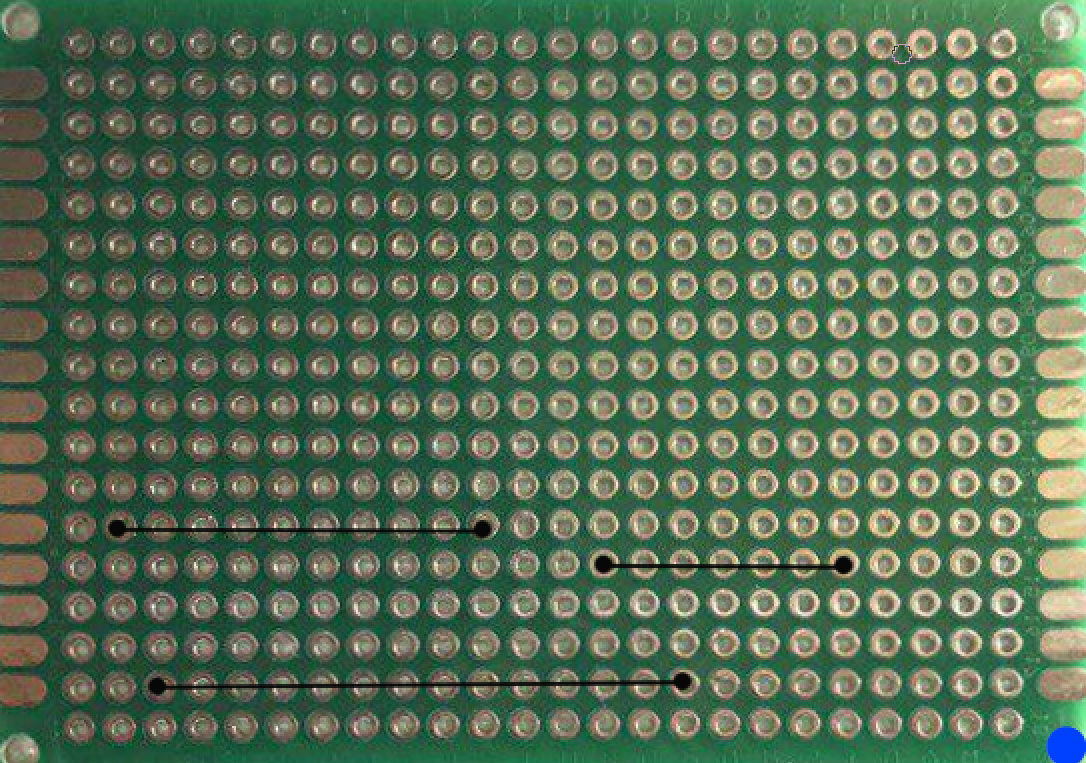
\includegraphics[width=0.8\textwidth]{img/dibujo_placa_vista_inferior_parte_trasera.png}
  \caption{Vista trasera de la placa, parte posterior.}\label{fig:placa-tras-inf}
\end{figure}

\begin{figure}
  \centering
  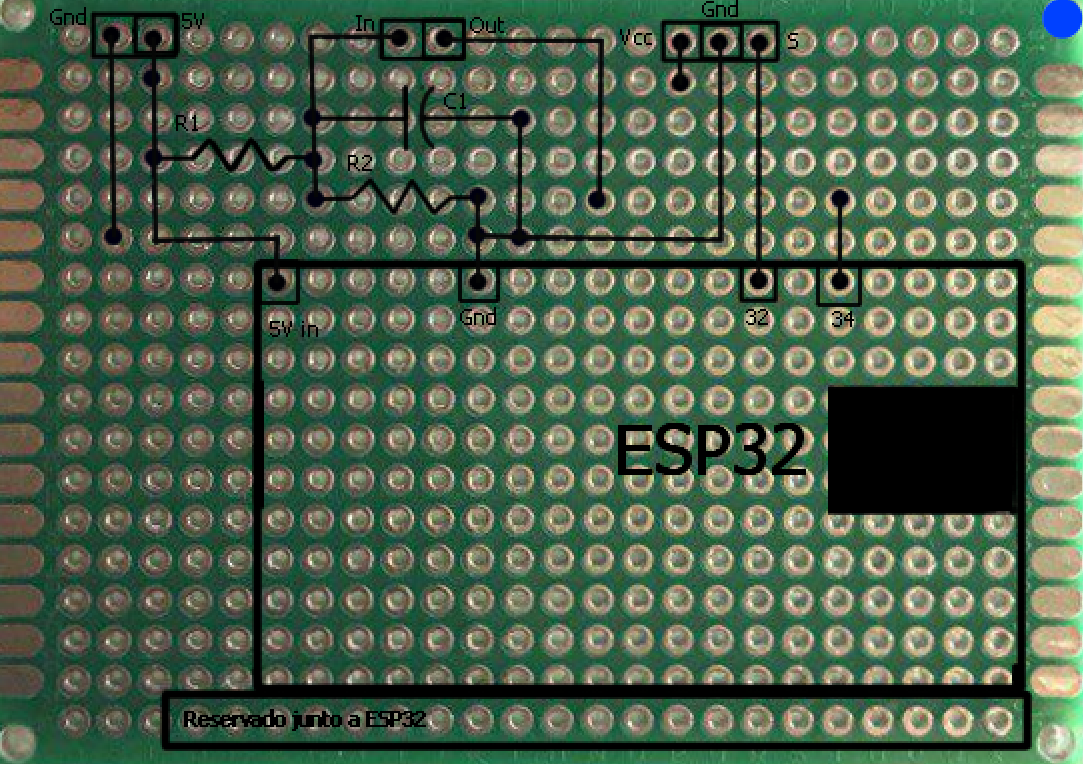
\includegraphics[width=0.8\textwidth]{img/dibujo_placa_vista_superior_parte_trasera.png}
  \caption{Vista trasera de la placa, parte posterior.}\label{fig:placa-sup-inf}
\end{figure}

Los adaptadores de los pines sobre los que se colocarán las otras
componentes queda dispuestos de acuerdo a la
Figura~\ref{fig:visual-adaptadores}. Hacemos uso de estos adaptadores
a fin de simplificar las tareas de mantenimiento y sustitución de
componentes en caso de avería.

\begin{figure}
  \centering
  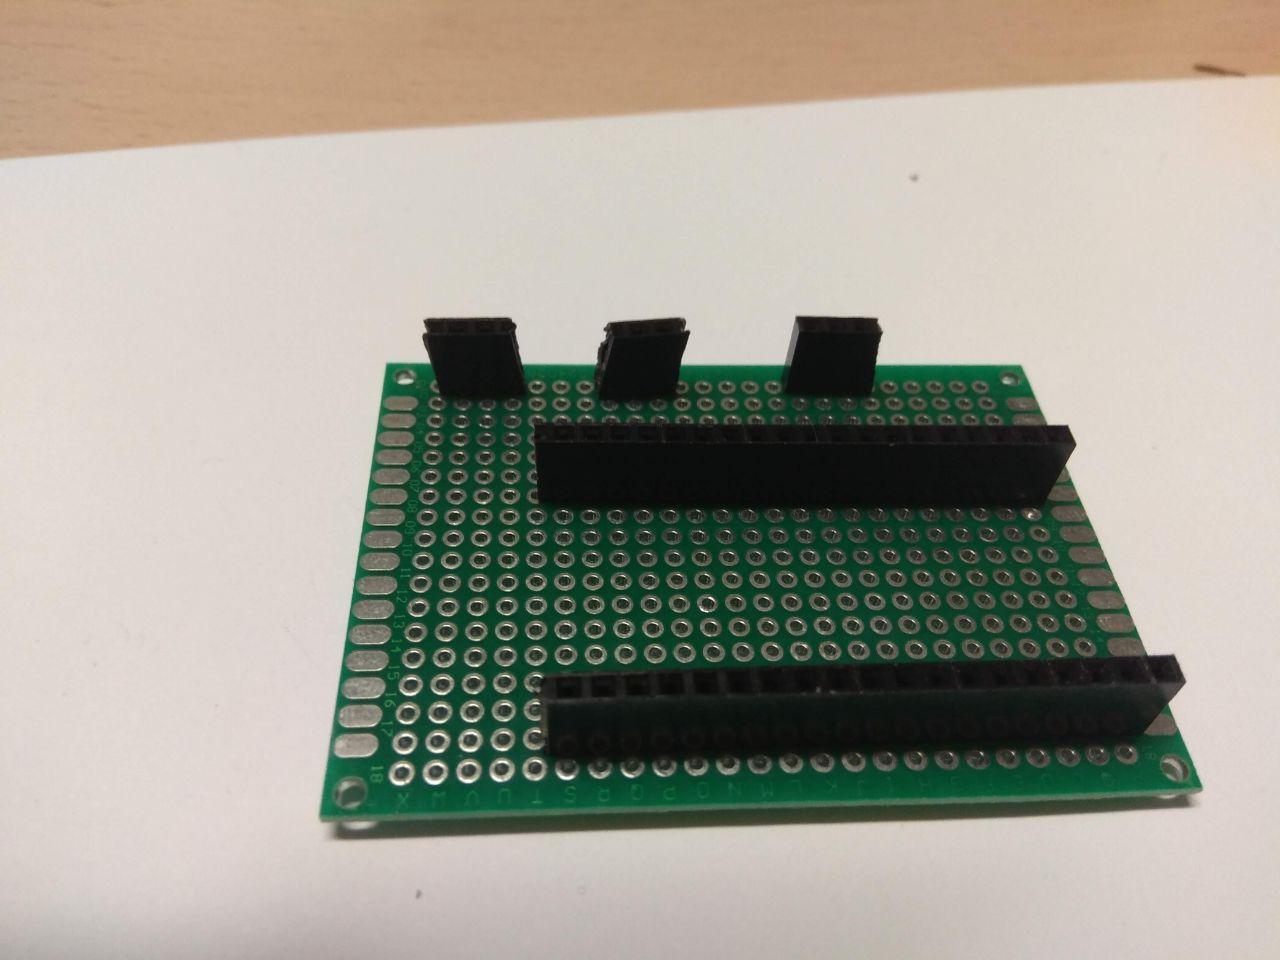
\includegraphics[width=0.8\textwidth]{img/placa_con_adaptadores_pines.jpg}
  \caption{Adaptadores de las componentes.}\label{fig:visual-adaptadores}
\end{figure}

El circuito resultante es el que podemos observar en las
figuras~\ref{fig:soldado_superior} y~\ref{fig:soldado_inferior}.

\begin{figure}
  \centering
  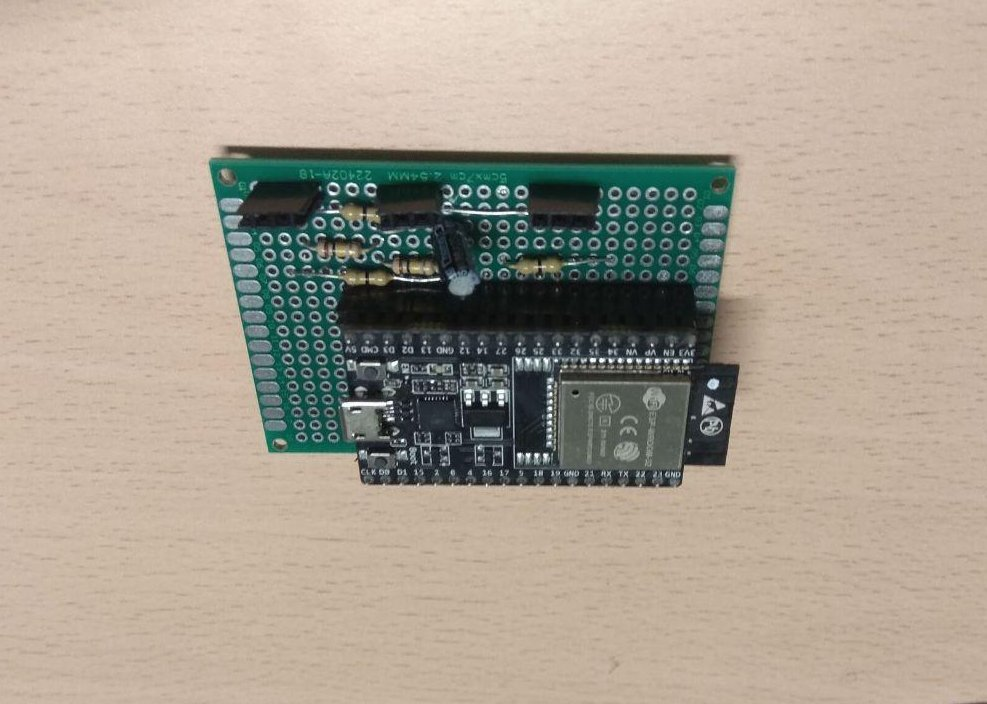
\includegraphics[width=0.8\textwidth]{img/soldadura_superior.jpg}
  \caption{Soldadura parte superior placa.}\label{fig:soldado_superior}
\end{figure}

\begin{figure}
  \centering
  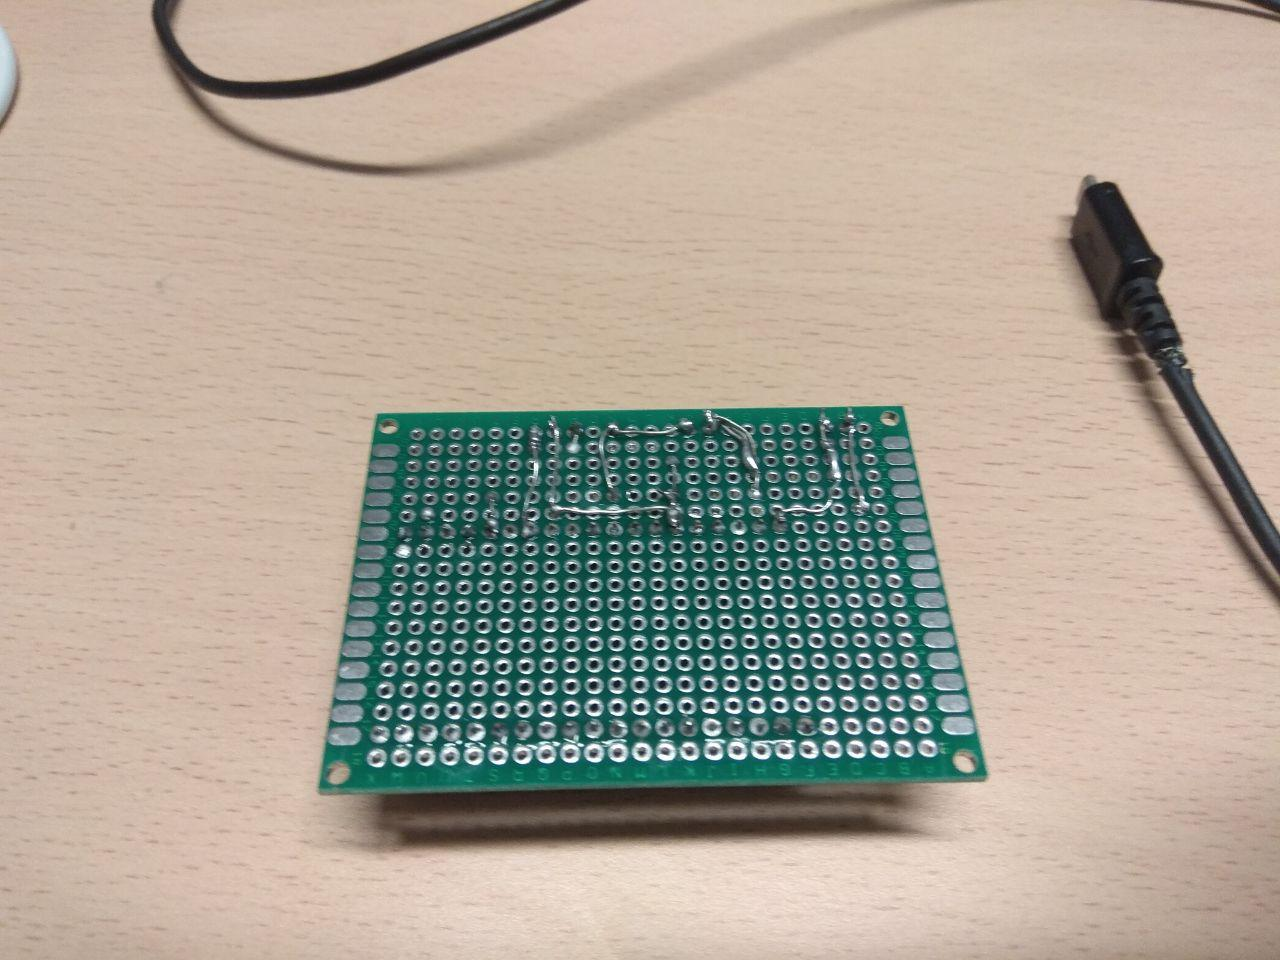
\includegraphics[width=0.8\textwidth]{img/soldadura_inferior.jpg}
  \caption{Soldadura parte inferior placa.}\label{fig:soldado_inferior}
\end{figure}

Tanto la alimentación como la medición de la corriente se produce a
partir de un cable que hemos seccionado y empalmado a las componentes
de nuestro circuito.

Para abstraer el diseño del enchufe y simplificar el uso del mismo al
usuario lo hemos acoplado en una caja de conexión. De este modo el
usuario final puede limitarse a, simplemente, conectar el dispositivo
a medir a nuestro enchufe inteligente y este a una fuente de
alimentación. Una conexión macho y una hembra.

\subsubsection{Programa del microcontrolador}

Toda la lógica del enchufe, tanto lecturas como comunicaciones, son
gestionadas por el programa del microcontrolador. Y resulta conveniente
comprender qué elementos hacen posible esta mecánica.

Por un lado se encuentra la configuración de la comunicación. Es
necesario conectarse a la red sobre la que se trabajará para poder
comunicarse con el broker, así que se requiere conocer SSID y
contraseña de la red en la que se trabajará. Del mismo modo la
información del broker, temas MQTT de suscripción o publicación y
credenciales tendrán que ser conocidos. Dada la licencia permisiva de
este proyecto y la flexibilidad de programación del módulo ESP32 no
habrá problema en entregar el sistema al usuario final en el estado de
uso inmediato o de permitir que este lo adapte a sus necesidades.

El enchufe publica el cálculo del consumo en un tema asociado a su
identificador en el broker y se suscribe a los canales de control para
gestionar su funcionamiento (actualmente manejo del relé, pero puede
extenderse a configuración de otros parámetros).

A fin de procesar la información del consumo cada enchufe está
identificado unívocamente por un identificador que puede ser adaptado
\textit{ad-hoc} (se podrían utilizar otros identificadores como el del propio
microcontrolador, pero se deja a opción del usuario para permitir
flexibilidad en la nomenclatura).

En el apartado de las lecturas es destacable cómo se han realizado los
cálculos.

En términos de electromagnetismo se define la potencia W (la variable
que utilizamos para medir el consumo) como:

\[W = V\cdot A\]

Siendo V el voltaje del circuito, 230 voltios en España, y A la
intensidad de la corriente que mide el sensor.

Con las mediciones del sensor de corriente calculamos la
media cuadrática. La corriente alterna fluctúa en torno a valores
positivos y negativos siguiendo un comportamiento sinusoidal. La
manera de calcular la intensidad que realmente está pasando es
obteniendo el valor eficaz. Este valor eficaz para la intensidad se
corresponde con el valor cuadrático
medio\cite{alcaldesanmiguelElectrotecniaInstalacionesElectricas2014}.

Para reducir hipotéticos picos de ruido se realiza un muestreo un
intervalo de tiempo fijo y se calcula el consumo durante ese período
de tiempo \textit{W} tomando como valor de la corriente \textit{A} la
media de las medidas en el muestreo.

\newpage

\subsection{Servidor central}\label{subsec:servidor-central}

En el centro de nuestra arquitectura de estrella se encuentra el
servidor central. Una Raspberry Pi 3 Modelo B que actúa como broker
entre los publicadores y suscriptores de MQTT, como mencionábamos
en~\ref{subsubsec:broker_mosquitto}, haciendo uso de Mosquitto para
gestionar las publicaciones y suscripciones a los temas.

La configuración de nuestro broker no permite la conexión anónima, es
decir, toda conexión requerirá usuario y contraseña. Permitirá la
persistencia de los mensajes que publiquen en sus temas y almacenará
otros tantos de depuración.

Es necesario que el broker esté activo y sea persistente a reinicios y
caídas. Por esto hay que configurarlo para que Mosquitto se lance en
cada inicio del servidor.

Este problema se puede abordar en un sistema Linux (y en particular en
Raspbian, el Sistema Operativo que estamos usando) de diversas
maneras. Una opción es usar el archivo \texttt{/etc/rc.local} para
ejecutar una orden en un script. Esta opción es similar al uso de un
\textit{cronjob} definido en cada inicio. También existe la
posibilidad de definir un servicio y activarlo al inicio con
\textit{systemd} (\textit{daemons}, procesos en segundo plano, del
sistema que se ejecutan al inicio). Cualquiera de estos métodos
resulta válido para esta finalidad.

Este servidor supone el nodo central de nuestra topología de red, es
por tanto el más determinante para el correcto funcionamiento del
sistema. Si quisiéramos mejorar la disponibilidad del sistema para
poder seguir utilizándolo aunque este servidor esté caído puede ser
una mejora utilizar un segundo servidor similar a este al cual el
resto de nodos tomaran por broker en caso de que el primero estuviera
inaccesible.

\subsubsection{Configuración de red}

Para favorecer la localización del servidor central en la red es
conveniente asignarle bien una IP estática (configurar alguna interfaz
o modificar la configuración del cliente dhcp en Raspberry Pi) o bien
utilizar algún DNS y que se actualice la dirección de la misma.

En este caso hemos asignado una IP estática al servidor dentro de
nuestra red y hemos solicitado un nombre de dominio que actualiza la
IP pública del router de acceso al servidor, configurando además un
reenvío de puertos para que un cliente pueda conectarse desde el exterior.


\begin{figure}[H]
  \centering
  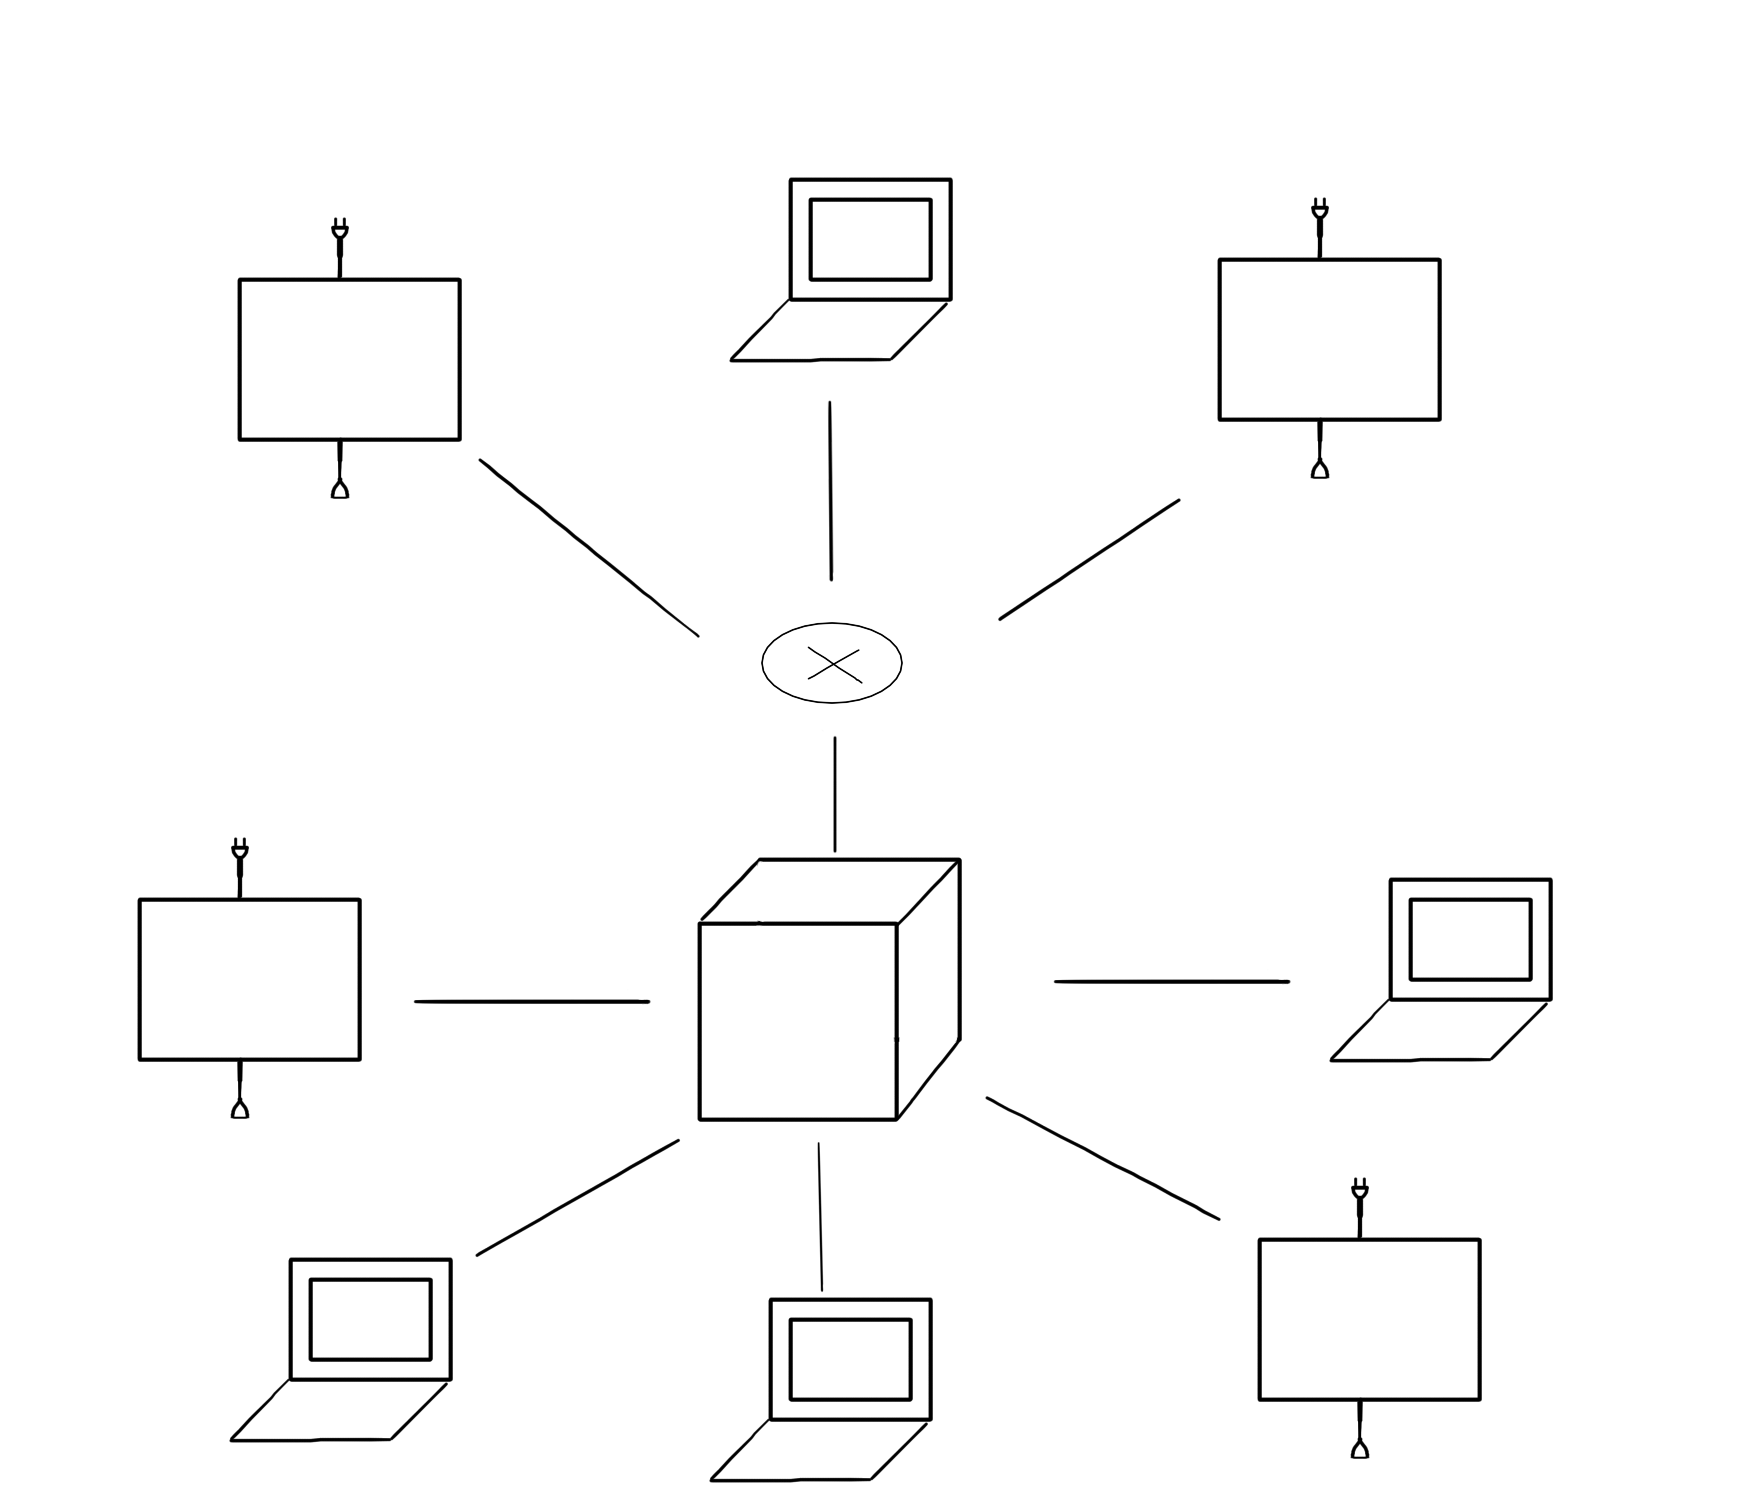
\includegraphics[width=0.9\textwidth]{img/esquema_estrella_internet.png}
  \caption{Esquema de la configuración de red y conexión a internet.}\label{fig:esquema-estrella-internet}
\end{figure}


Como hemos indicado previamente los nodos periféricos se conectarán
con el servidor central. Pero resulta interesante estudiar cómo se
producen estas conexiones de acuerdo a la configuración de red.

En la Figura~\ref{fig:esquema-estrella-internet} podemos ver un
esquema de cómo se realizan las conexiones. Aquellas que están
directamente conectadas con el servidor central representan elementos
en la red local, cuya conexión no desentraña ninguna complejidad. Sin
embargo, aquellas que se encuentran conectadas a un nodo intermedio
representan las conexiones provenientes desde redes externas. Desde
internet. Y se pueden comunicar con el servidor central mediante el
router (nodo intermedio) que debe tener la configuración oportuna de
reenvío de puertos.

\subsubsection{Gestión de la base de datos}

En un primer diseño ubicamos la base de datos en los propios usuarios
finales, de modo que libraríamos al servidor central de mayor carga de
gestión y limitaríamos las comunicaciones en la red a publicaciones y
suscripciones de MQTT. Esta idea fue descartada finalmente pues
resulta más valioso tener una base de datos sin inconsistencias entre
los distintos almacenamientos de los clientes que un servidor menos
congestionado.

En el diseño final, en el servidor central se encuentra situada una
base de datos donde se recogen las lecturas de los enchufes. De este
modo se puede gestionar la difusión de esta información a los clientes
sin comprometer la consistencia de los datos.

La estructura de esta base de datos consiste en una tabla que
incorpora para cada medición una fila con los datos del enchufe en el
que se ha leído, el consumo y la hora registrada según el servidor. La
creación de esta base de datos se gestiona con un programa que crea
una base de datos con este esquema si no existía previamente. El
Sistema Gestor de Bases de Datos usado ha sido
sqlite\cite{SQLiteHomePage} por su capacidad para implementar una base
de datos relacional SQL sencilla y rápida.

La manera en la que se pobla esta base de datos es mediante un
programa que se ejecuta de manera concurrente al broker y que se
comporta como un suscriptor más al tema de las publicaciones de
consumo. Pero su procesamiento del mensaje implica su almacenamiento
en la base de datos.

\subsubsection{Consulta a la base de datos}\label{subsubsec:consulta-api}

Una vez que la información del consumo energético de nuestros enchufes
se encuentra almacenada en una base de datos en nuestro servidor
central es necesario implementar algún medio de comunicación entre el
servidor y el usuario final para que puedan acceder a esta
información.

La solución que le hemos dado a este requisito es la creación de una
API simple, un microservicio. Una interfaz que sirva a un usuario para
consultar la información relativa a un enchufe. Todas las peticiones
que se pueden hacer a esta API son exclusivamente de consulta
(peticiones HTTP tipo GET), por lo que no existe el riesgo de que
múltiples escritores generen problemas derivados de un acceso
concurrente.

Esta API está optimizada para realizar las consultas a la base de
datos de modo que se adecúen a los procesos en otros módulos para
evitar un postprocesado innecesario en etapas posteriores. Ofreciendo
los datos relativos a uno o varios enchufes y a un rango determinado
de lecturas en un formato específico que sea más directamente
interpretable por las aplicaciones que se comuniquen con la API.

\newpage

\subsection{Aplicación de escritorio}

El último eslabón de nuestro sistema es el cliente de escritorio. Una
aplicación que permite al usuario final interactuar con el resto del
sistema.

Este cliente es en realidad una interfaz que otorga control sobre las
funcionalidades del sistema: Por un lado, acceder a la información
sobre el consumo eléctrico y visualizarla y, por otro lado, manipular
los enchufes inteligentes para controlar su estado.

En la topología de nuestro diseño este tipo de nodo forma parte de los
nodos periféricos que se conectan al servidor central. Pero a
diferencia de los otros nodos periféricos, los enchufes inteligentes,
estos permiten una mayor flexibilidad y libertad de configuración. Por
esto se le permite al cliente modificar desde la aplicación los
parámetros de conexión.

\begin{figure}[H]
  \centering
  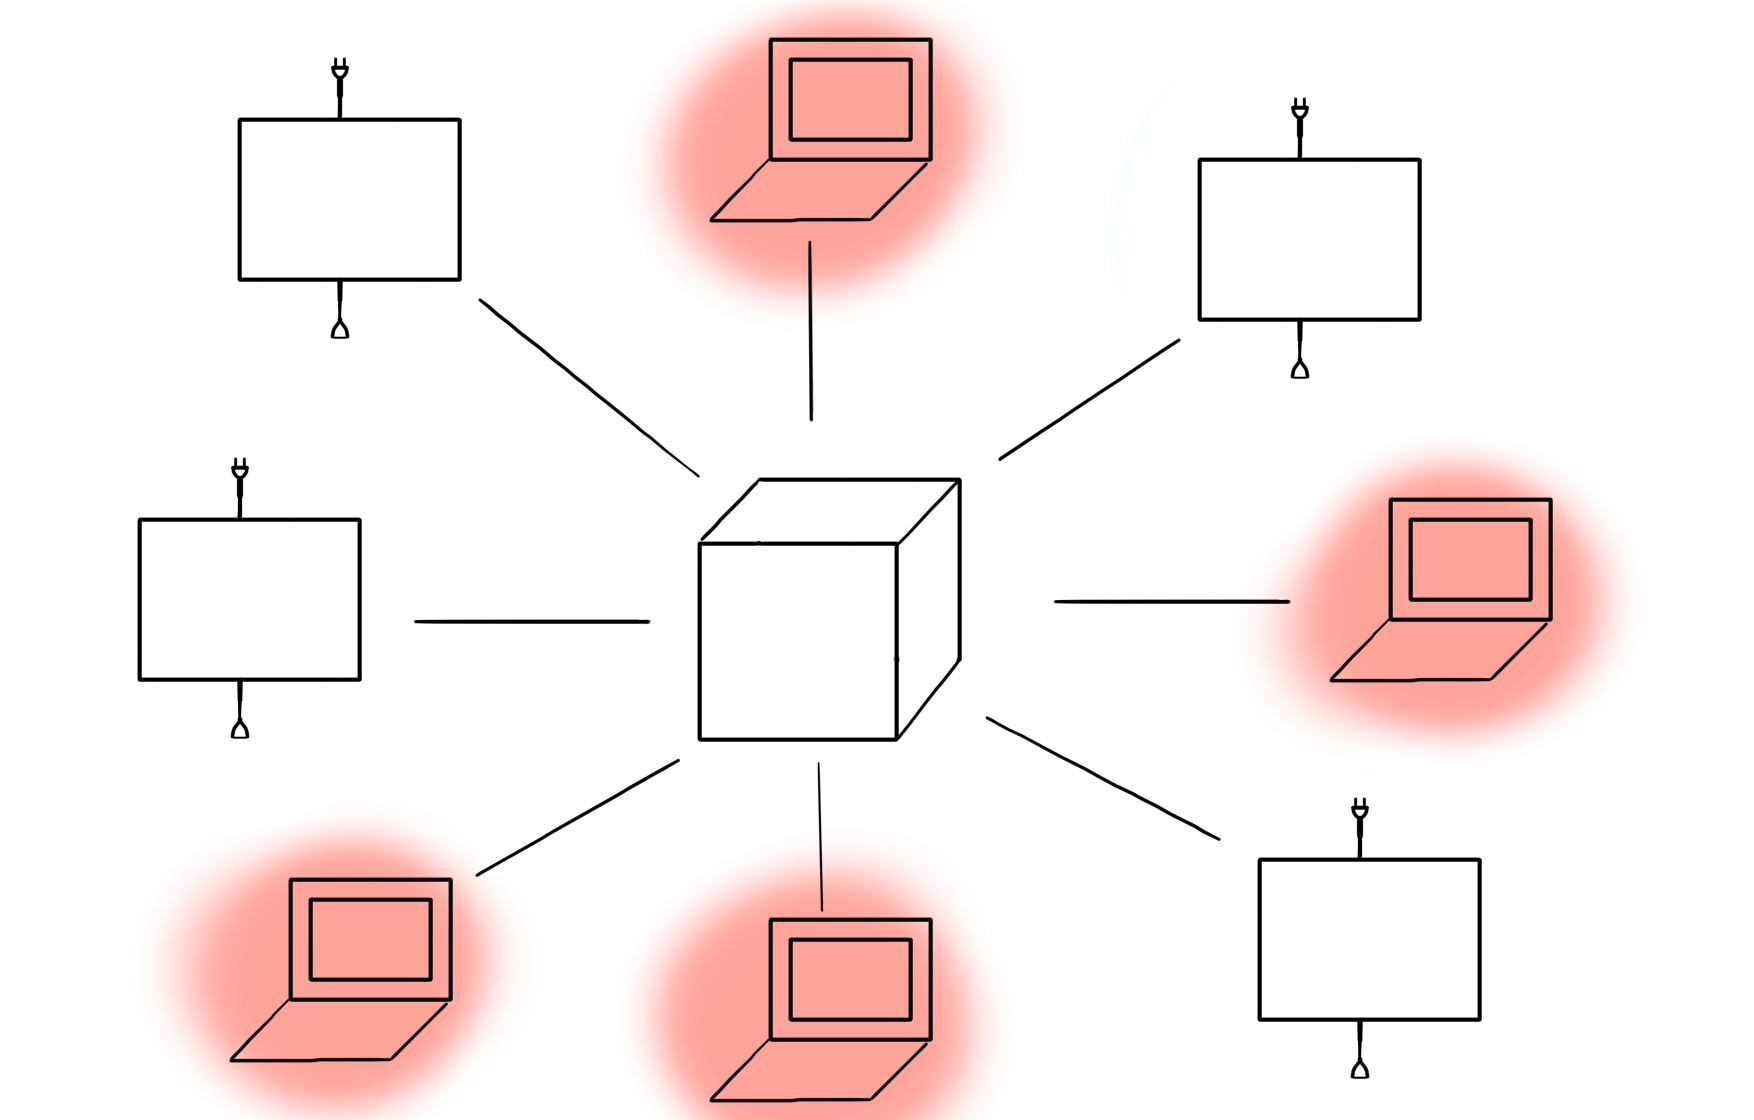
\includegraphics[width=0.9\textwidth]{img/esquema_estrella_nodos_finales_coloreados.png}
  \caption{Topología del sistema, en rojo los clientes de escritorio.}\label{fig:esquema-estrella-color}
\end{figure}


Una vez conectado al servidor la aplicación puede obtener la
información del mismo. Consultar su base de datos para obtener el
consumo realizado y poder visualizarlo de manera sencilla o consultar
los registros en mayor profundidad.

Al obtener esta información también estamos consultando qué enchufes
se encuentran conectados y qué identificadores tienen. Lo cual nos
permitirá controlar el estado de los enchufes (modificando el estado
de su relé) publicando en el broker en los temas de control a los que
los enchufes estarán suscritos.

A continuación se adjuntan algunas imágenes de la interfaz junto a una
descripción de su utilidad:

\begin{figure}[H]
  \centering
  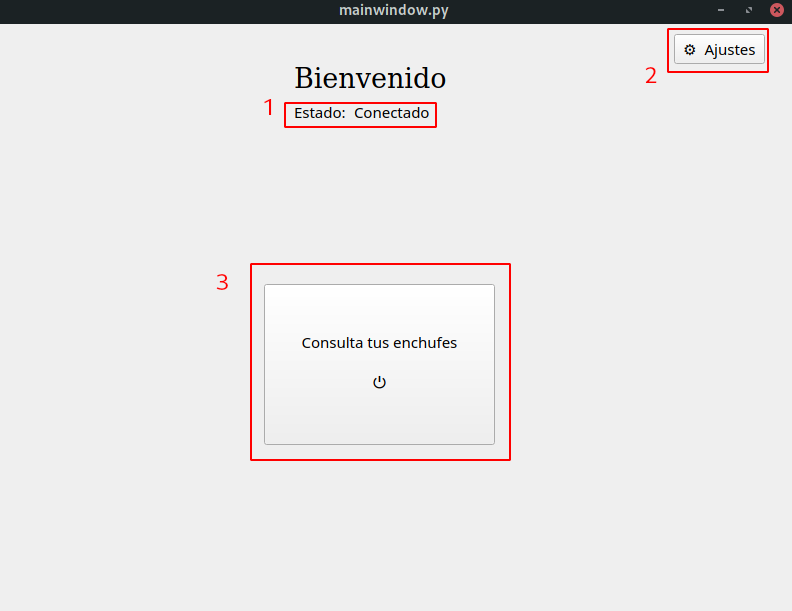
\includegraphics[width=0.9\textwidth]{img/interfaz_main_window.png}
  \caption{Ventana principal.}\label{fig:interfaz-main}
\end{figure}

Esta interfaz permite:

\begin{enumerate}
\item{Conocer el estado de conexión actual con el broker}
\item{Acceder a la configuración de comunicación con el broker}
\item{Acceder a una lista con los enchufes accesibles}
\end{enumerate}

\begin{figure}[H]
  \centering
  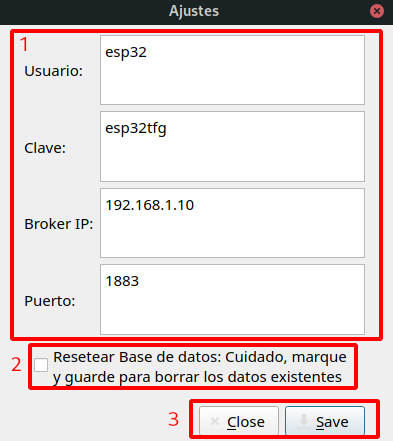
\includegraphics[width=0.6\textwidth]{img/interfaz_settings_window.png}
  \caption{Ventana de ajustes.}\label{fig:interfaz-settings}
\end{figure}

En la ventana de configuración se permite:

\begin{enumerate}
\item{Modificar parámetros de configuración de red}
\item{Restablecer configuración por defecto}
\item{Guardar o cancelar los cambios realizados}
\end{enumerate}

\begin{figure}[H]
  \centering
  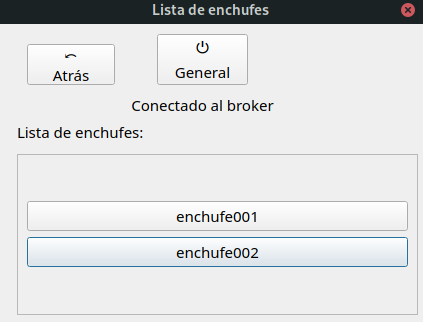
\includegraphics[width=0.6\textwidth]{img/interfaz_plug_list.png}
  \caption{Lista de enchufes accesibles.}\label{fig:interfaz-plug-list}
\end{figure}

En esta ventana se muestra una lista de enchufes que se actualizan
dinámicamente según se van conectando más enchufes al sistema. Permite
acceder al control de cada enchufe pero también ofrece una opción para
analizar y controlar simultáneamente todos los enchufes conectados al
sistema.

La visualización de cada enchufe es la siguiente:

\begin{figure}[H]
  \centering
  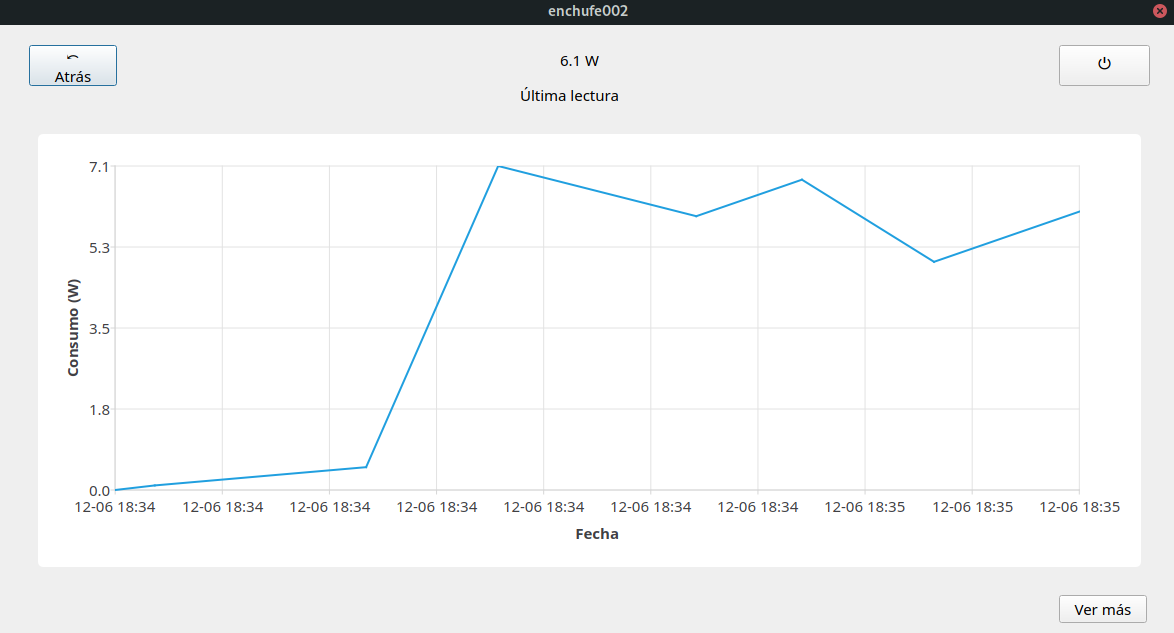
\includegraphics[width=1\textwidth]{img/interfaz_graphics.png}
  \caption{Ventana de un enchufe.}\label{fig:interfaz-graphics}
\end{figure}

En esta vista se permite visualizar de manera rápida el consumo para
cada enchufe (o para todos si se accede desde la opción
general). Además se ofrece información exacta sobre el estado actual
mostrando la última lectura, se permite el control individual con el
interruptor de la parte superior derecha y se permite acceder a un
registro en detalle del consumo de este enchufe con el botón
\textit{Ver más} en la parte inferior derecha.

\begin{figure}[H]
  \centering
  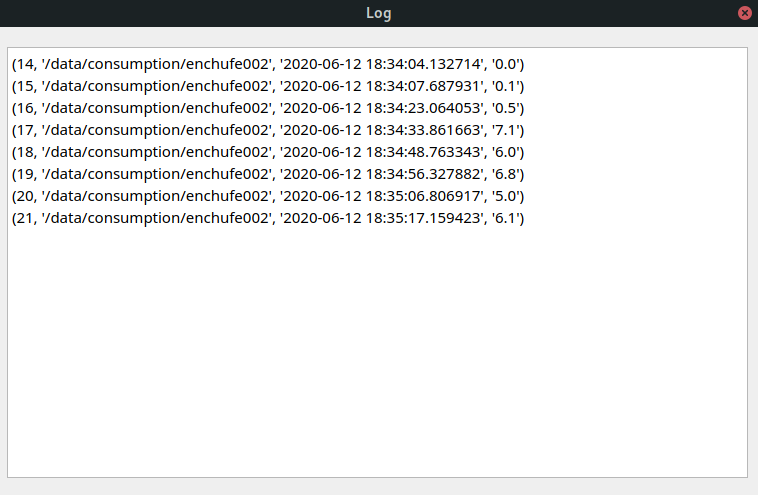
\includegraphics[width=0.9\textwidth]{img/interfaz_log.png}
  \caption{Log en detalle del consumo de un enchufe.}\label{fig:interfaz-log}
\end{figure}


\newpage

\section{Pruebas y test}\label{tests}

En el desarrollo de cualquier software es determinante asegurarse de
que el código funcionará siempre en el contexto del sistema a pesar de
que se introduzcan cambios en el propio código. La salida debe ser la
esperada a pesar de avanzar en el desarrollo del producto.

Nuestro sistema, igualmente, necesita que el desarrollo sea pautado
por unas pruebas o \textit{tests} que nos garanticen que lo que
estamos haciendo efectivamente es lo que deseamos obtener.

La particularidad a la hora de realizar \textit{tests} en un sistema
tan complejo reside en que cada elemento del sistema debe
individualmente asegurarse de su correcto funcionamiento y debe
existir algún tipo de prueba que compruebe que los componentes se
están integrando y comunicando debidamente.

\subsection{Pruebas en el módulo WiFi}

En primer lugar analizaremos el proceso de prueba para el módulo
WiFi. En realidad este subsistema al ser en esencia un
microcontrolador se puede analizar como un sistema embebido como
también pasa con Arduino.

Existen varias alternativas para realizar tests unitarios para
Arduino o ESP32~\cite{murdochMmurdochArduinounit2020,
  salmenrinneSusundbergArduinosimpleunittest2019}. Algunas orientadas
a la ejecución en la propia placa y la comunicación por puertos
seriales y otras orientadas a la simulación por software de la
placa. En cualquier caso herramientas que se encuentran en desarrollo
y que distan de ser una solución consolidada.

Ambos métodos tienen sus carencias, ejecutar en una placa conlleva
ocupar el uso de una placa en todo momento del desarrollo y puede
ralentizar el avance por los tiempos de carga del programa e
interpretación de los resultados obtenidos por serial. El proceso de
simulación, si bien consigue ser más rápido, pues un procesador de un
ordenador personal resulta de órdenes de magnitud más rápido que un
microcontrolador, tiene dos inconvenientes principales: Por un lado la
complejidad de la simulación, debes adaptar las clases y estructuras
de datos a las que necesitaría tu programa (requisitos para simular
seriales, por ejemplo) y, por otro lado, careces del acceso real a
sensores u otros elementos que puedan estar influyendo en la salida de
tu sistema.

Sea cual sea el método utilizado es necesario tener en cuenta que un
sistema embebido puede fallar por múltiples razones y no nos va a
garantizar el correcto funcionamiento. El objetivo será garantizar que
el comportamiento sea correcto o, al menos, consistente en los errores
(esperado).

En nuestro caso hemos hecho probado que el microcontrolador funcione
adecuadamente simulando los valores obtenidos por los
sensores. Nuestro objetivo es garantizar el correcto funcionamiento
del programa del microcontrolador, asumiendo que los sensores
funcionarán bien.

\newpage

\subsection{Pruebas en el servidor central}

En el servidor central se sitúan dos elementos principales: El broker
de Mosquitto, que es un software externo pero que podríamos usar para
probar efectiva integración de este con enchufes y clientes finales; y
la API que envuelve la funcionalidad de consulta de la base de datos,
que debe ser debidamente probado.

Para comprobar el debido funcionamiento de los módulos en esta parte
hemos realizado un conjunto de pruebas mediante una herramienta
genérica de tests unitarios (\textit{unittest} y \textit{pytest}
en Python).

Algunos de estos tests en el servidor han sido comprobar la creación
de la base de datos o el comportamiento ante los errores de conexión
del módulo al broker.

Estos nos han servido para diseñar mejor la conducta de este
sistema. Por ejemplo se encontró el problema de que el programa no
podía continuar su ejecución si el broker no estaba
disponible. Captando la excepción oportuna en uno de los tests
elaborar un comportamiento que mejorara la estabilidad del servidor.

\begin{figure}[H]
\begin{lstlisting}
test_create_database
.test_connection
.
----------------------------------------------------------------------
Ran 2 tests in 5.038s

OK
\end{lstlisting}

\caption{Salida de la ejecución los tests creados en el servidor}
\end{figure}

\newpage

\subsection{Pruebas en la aplicación de escritorio}

Nuestra aplicación de escritorio también consta de dos elementos que
resultan de interés: La interfaz de usuario y los módulos que dan
soporte a la lógica de la aplicación.

Realizar tests sobre una interfaz de usuario puede resultar ser una
tarea menos habitual en nuestro ámbito de trabajo usual, de hecho no
suele ser suficiente utilizar una herramienta genérica. Por suerte
existen herramientas específicas para comprobar el correcto
funcionamiento de la interfaz de usuario. Este es el caso de la
biblioteca que hemos utilizado, que dispone de una herramienta
realizar test específicos tales como creación de elementos, contenido
de campos o simulación de acciones (\textit{QTest} para
\textit{PySide2}, en Python).


\begin{figure}[H]
\begin{lstlisting}
.test_main_window_creation
.test_plug_list_window
.test_plug_window
.test_check_connection
.test_get_from_db
.test_get_settings
.test_load_scene
.
----------------------------------------------------------------------
Ran 8 tests in 21.578s

OK

\end{lstlisting}

\caption{Salida de la ejecución los tests creados para la app}
\end{figure}

Para esta parte hemos tenido que comprobar múltiples apartados: La
creación de la interfaz, su correcto funcionamiento y la funcionalidad
de los módulos que se usan para dar soporte al subsistema de la
aplicación de escritorio.


\newpage

\section{Conclusión}\label{conclusion}

Ya sabíamos que el Internet de las Cosas traía consigo innumerables
posibilidades para extender la concepción habitual de los objetos que
nos rodean en nuestro día a día.

Con este proyecto se pretende hacer ver que el Internet de las Cosas
no es un concepto distante y que no existe una barrera económica o
tecnológica que solo permita a grandes empresas trabajar con él. El
Internet de las Cosas es accesible para cualquiera tanto para su uso
como para su desarrollo. Apto para cualquiera sin requerir grandes
gastos económicos y con unas opciones de diseño y desarrollo que
existen y que cada vez están mejor documentadas.

Entre los retos que se han planteado en este trabajo se encuentran
trabajar con fundamentos de la física, comprender las utilidades de
muchas componentes electrónicas que hemos acabado usando en nuestro
diseño y que no son la materia de estudio usual que se puede encontrar
un Ingeniero Informático en su trabajo pero que, sin embargo, debemos
ser capaces de trabajar con ellos si la ocasión lo requiere. Lo cual
nos enseña que la informática, y en particular en el ámbito del IoT,
es un área que intersecta con muchas otras ramas del conocimiento como
la física, la bioinformática o la medicina entre muchas otras. Y esto
implica que debemos ser capaces de adaptar nuestros conocimientos para
extenderlos a cualquier problema que se nos presente.

Otro de los retos que se han presentado y que es destacable es, en sí
mismo, el diseño de un sistema tan grande. En muchas ocasiones nos
especializamos en aprender a trabajar en campos muy concretos de la
informática, inteligencia artificial, desarrollo de software, sistemas
de información, etc. Pero para hacer proyectos reales por cuenta
propia es necesario abarcar áreas que se escapan de la especialidad de
cada uno. Ese ha sido uno de los motivos que me impulsó a hacer este
trabajo, enfrentarme a una placa base sobre la que diseñar un circuito
y soldar un microcontrolador, planificar unas bases de datos,
gestionar la comunicación y elaborar la interfaz de un usuario
final. En resumen, llevar un diseño de principio a fin, contemplando
todas las posibilidades de diseño a la par que se investiga sobre
aquellas que se desconocen.

Por este último motivo han surgido desafíos derivados. La importancia
de establecer un desarrollo basado y dirigido por tests es un tema que
en nuestra formación se ha procurado tener presente. Está claro que si
se quiere desarrollar un software de calidad y escalable es vital
establecer este paradigma de desarrollo. Sin embargo el ámbito de este
proyecto ha sido amplio y ha resultado una dificultad procurar
elaborar un conjunto de pruebas o tests que verifiquen el correcto
desarrollo del proyecto y la calidad del mismo. Esto me ha permitido
conocer más de cerca cómo se realiza este desarrollo en otros ámbitos
menos usuales y, aunque se pueda mejorar la calidad del mismo,
establecer una buena aproximación.

Considero este proyecto como una oportunidad de aprender y de
desarrollo personal como Ingeniero Informático, pero también espero
que sirva de utilidad a quien quiera monitorizar el consumo en su
hogar pero no enfrentarse a todo el proceso de diseño y sobre todo de
inspiración a quien quiera desarrollar un proyecto \textit{maker},
autónomo y al alcance de su mano, para demostrar que simplemente con
la voluntad por aprender y un trabajo de investigación se puede llegar
a conseguir lo que se proponga.

\newpage

\appendix
\section{Anexo: Código del proyecto}

Todo el código del proyecto puede ser consultado en este repositorio de Github:

\href{https://github.com/jojelupipa/smart-plug}{https://github.com/jojelupipa/smart-plug}

El repositorio se ha estructurado de manera que se pueda consultar
fácilmente cada sección de este trabajo (accesible a continuación mediante hiperenlace):

\begin{itemize}
\item{\href{https://github.com/jojelupipa/smart-plug/tree/master/src}{\textbf{Código fuente:}}}
  \subitem{\href{https://github.com/jojelupipa/smart-plug/blob/master/src/esp32_module/esp32_module.ino}{Enchufe inteligente}}
  \subitem{\href{https://github.com/jojelupipa/smart-plug/tree/master/src/server}{Servidor central}}
  \subsubitem{\href{https://github.com/jojelupipa/smart-plug/blob/master/src/server/requirements.txt}{Dependencias (Python) del servidor}}
  \subsubitem{\href{https://github.com/jojelupipa/smart-plug/blob/master/src/server/script_provisionammiento.sh}{Provisionamiento del servidor}}
  \subsubitem{\href{https://github.com/jojelupipa/smart-plug/blob/master/src/server/mosquitto.conf}{Configuración Mosquitto}}
  \subitem{\href{https://github.com/jojelupipa/smart-plug/tree/master/src/app}{Aplicación de escritorio}}
  \subsubitem{\href{https://github.com/jojelupipa/smart-plug/blob/master/src/app/requirements.txt}{Dependencias de la app}}
\item{\href{https://github.com/jojelupipa/smart-plug/tree/master/documentacion}{\textbf{Documentación:}}}
  \subitem{\href{https://github.com/jojelupipa/smart-plug/tree/master/documentacion}{Memoria del proyecto}}
  \subitem{\href{https://github.com/jojelupipa/smart-plug/blob/master/documentacion/biblio.bib}{Bibliografía del proyecto}}
\end{itemize}

\newpage

\section{Anexo: Cómo usar este proyecto}

En el \href{https://github.com/jojelupipa/smart-plug}{repositorio del
  proyecto} se recogen instrucciones de uso de cada una de las partes
del sistema. En esta sección se busca proporcionar unas pautas para
que el usuario pueda sacarle el máximo partido al sistema.

Dada la modularidad de este proyecto puede usarse en su
conjunto o simplemente las partes que se necesiten, modificando el
resto o sustituyéndolas por otras partes que resulten más
convenientes.

Además, dada la licencia permisiva de este proyecto, se deja la
libertad al usuario de modificar el diseño del sistema para que se
adecue a sus necesidades.

Para este fin se adjuntan algunas indicaciones con los aspectos más
relevantes a tener en cuenta si se desea integrar el sistema con otros
elementos.

\subsection{Enchufe Inteligente}

Usar el enchufe diseñado en este proyecto es, simplemente, una
simplificación del trabajo. Es posible que no se dispongan de los
materiales necesarios para construir este mismo enchufe, que se
tuviera previamente otro enchufe o que se prefiera usar algún otro
tipo de comunicador.

Cualquier sensor, enchufe o interfaz que actúe como transmisor debe
hacer uso de un cliente MQTT que publique en el tema (\textit{topic})
indicado.

\texttt{/data/consumption/*nombre\_enchufe*}

\textit{Sustitúyase *nombre\_enchufe* por el identificador de la
  interfaz a conectar}

Del mismo modo, si se desea dotar de una funcionalidad de control
sobre el enchufe este deberá contener algún tipo de relé o interruptor
que se controle mediante una suscripción al tema de control:

\texttt{/control/toggle/*nombre\_enchufe*}

\subsection{Servidor central}

Tampoco es necesario utilizar Mosquitto, mientras las credenciales
utilizadas por los nodos finales (enchufes y clientes finales) sean
las apropiadas para la comunicación el broker utilizado no será un
problema para el correcto flujo de la información.

\subsection{Cliente de escritorio}

El cliente de escritorio puede ser adaptado también a las necesidades
del usuario, la obtención de información se hace mediante un conjunto
de consultas a la API del servidor central. Por lo que todas las
vistas pueden ser modificadas como se desee.

La manipulación de los enchufes se realiza mediante publicaciones MQTT
al tema correspondiente en el broker:

\texttt{/control/toggle/*nombre\_enchufe*}

\newpage

\bibliographystyle{unsrt}
\begingroup
\raggedright%

\bibliography{biblio} 
\endgroup

\end{document}
